\documentclass{article}
\usepackage[utf8]{inputenc}
\usepackage{amsmath}
\usepackage{amssymb}
\usepackage{amsthm}
\usepackage{cancel}
\usepackage{color,soul}
\usepackage{comment}
\usepackage{graphicx}
\usepackage{hyperref}
\usepackage{listings}
\usepackage{outlines}
\usepackage{subcaption}
\newcommand{\lands}{\:\land\:}                          % "logical and with spaces". Pone el "y" dejando espacio(mediano) a los costados
\newcommand{\comma}{,\,}                                % Pone la coma seguida de un espacio(chiquito)
\newcommand{\tq}{/\,}                                   % "tal que". Pone la barrita del "tal que" seguida de un espacio
\newcommand{\vees}{\:\vee\:}                            % "vee with spaces". Pone el "ó" con espacio a los costados
\newcommand{\eq}{\:=\:}                                 % Pone el igual con espacios(medianos) a los costados
\newcommand{\neqs}{\:\neq\:}                            % Pone el desigual con espacios(medianos) a los costados
\newcommand{\relates}{\mathcal{R}}                      % Pone la R para denotar cuando un elemento se realciona con otro
\newcommand{\enteros}{\mathbb{Z}}                       % Pone la Z de los números enteros
\newcommand{\naturales}{\mathbb{N}}                     % Pone la N de los números naturales
\newcommand{\racionales}{\mathbb{Q}}                    % Pone la Q de los números racionales
\newcommand{\complejos}{\mathbb{C}}                     % Pone la C de los números complejos
\newcommand{\cuerpo}{\mathbb{K}}                        % Pone la K para denotar un cuerpo (los cuerpos son R,Q o C)
\newcommand{\reales}{\mathbb{R}}                        % Pone la R de los números reales
\newcommand{\vabs}[1]{\left\lvert #1 \right\rvert }     % Pone el módulo y recibe como argumento el número
\newcommand{\Rightarrows}{\: \Rightarrow \:}            % Pone la flecha del "entonces" con espacios(medianos) a los costados
\newcommand{\Leftrightarrows}{\: \Leftrightarrow \:}    % Pone la flecha del "si y solo si" con espacios(medianos)
\newcommand{\existsuniq}{\exists !\,}                   % Pone el "existe un único" dejando un espacio(chiquito) para que no quede tan amontonado
\newcommand{\bld}[1]{\textbf{#1}}
\newcommand{\sumatoria}[2]{\sum_{#1} ^{#2}}
\graphicspath{{./Images/}}
%\DeclareUnicodeCharacter{2212}{\textendash}

\title{Matematica Discreta}
\author{Nicolás Margenat}
\date{1Q 2021}


\begin{document}
\maketitle
\tableofcontents

\newpage
\section{Grafos}
\subsection{Definciones Previas}
\subsubsection*{Definición 1. Grafo}
Un grafo $G=(V,E)$ es una estructura matemática que consta de dos conjuntos V y E.
Los elementos de V se llaman vértices o nodos y los elementos de E se llaman aristas.
Cada arista tiene un conjunto de uno o mas vértices asociados que se llaman puntos extremos.
($V \neq \varnothing$)

\subsubsection*{Definición 2. Grafo Trivial}
$\#V=1 \lands \#E=0$

\subsubsection*{Definición 3. Lazo}
Es una arista cuyos puntos extremos son coincidentes.

\subsubsection*{Definición 4. Arista propia}
Es una arista que no es un lazo.

\subsubsection*{Definición 5. Multigrafo}
Un grafo $G=(V,E)$ es un multigrafo si $\exists a \lands b \in V$ con 2 o mas aristas incidentes en $a$ y $b$. 
Caso contrario se llama $grafo$ $simple$.

\subsubsection*{Definición 6. Grafo dirigido o digrafo}
Es un grafo que tiene todas sus aristas dirigidas.

\subsubsection*{Definición 7. Multigrafo dirigido}
Un grafo $G=(V,E)$ es un multigrafo si $\exists a, b \in V$ con 2 o mas aristas de la forma $(a,b)$. 
Caso contrario se llama $digrafo$ $simple$.
\\CUIDADO: $(a,b) \neq (b,a)$

\subsubsection*{Definición 8. Matriz de incidencia}
La matriz de incidencia de un grafo $G$ es la matriz $I_G$ cuyas filas y columnas son indexadas por algun orden
de $V_G$ y $E_G$ respectivamente, tal que:
\begin{equation*}
    I_G[v,e]=
    \begin{cases}
        0 &\text{si v no es un extremo de e;} \\
        1 &\text{si v es un extremo de e;} \\ 
        2 &\text{si e es un lazo en v.}
    \end{cases}
\end{equation*}
Si es un digrafo;
\begin{equation*}
    I_D[v,e]=
    \begin{cases}
        0 &\text{si v es un extremo de e;} \\
        1 &\text{si v es la cabeza de e;} \\ 
        -1 &\text{si v es la cola de e;} \\ 
        2 &\text{si e es un lazo en v.}
    \end{cases}
\end{equation*}
\underline{Apuntes}:
\begin{itemize}
        \item Filas=vértices / Columnas=aristas
        \item $I_G$ es de $\#V \times \#E$
        \item Grafos: Cada columna suma como máximo 2, pues cada arista tiene como máximo 2 vértices. La fila no tiene restricción.
        \item Digrafos: Cada columna suma 2(lazo) o suma 0(dirigido a una dirección).
\end{itemize}

\subsubsection*{Definición 9. Matriz de Adyacencia}
La matriz de adyacencia de un grafo $G$ es la matriz $A_G$ cuyas filas y columnas son indexadas por algun orden de $V_G$, tal que:
\begin{equation*}
    A_G[u,v]=
    \begin{cases}
        \text{la cantidad de aristas entre ellos si} &u\neq v; \\
        \text{la cantidad de lazos si} &v = u
    \end{cases}
\end{equation*}
Si es un digrafo:
\begin{equation*}
    A_D[u,v]=
    \begin{cases}
        \text{la cantidad de aristas desde u hasta v si} &u\neq v; \\
        \text{la cantidad de lazos si} &v = u
    \end{cases}
\end{equation*}
\underline{Apuntes}:
\begin{itemize}
    \item $A_G = \#V \times \#V$
    \item Fila=Vértice / Columna=Vértice
    \item Grafo simple: Siempre son simétricos.
    \item Digrafo: NO son simétricos, si lo fuese estaríamos ante un grafo simple.
\end{itemize}
\underline{Observaciones}:
\begin{itemize}
    \item Sea $G$ un grafo con una matriz de adyacencia $A_G$.
    Entonces $A_G^r(u,v)$ es igual a \emph{la cantidad de caminos $u-v$ de longitud r}
    (Notar que $A_G^r(u,v)$ significa tomar el elemento $(u,v)$ de la matriz de adyacencia elevada a la r).
    \item Sea $D$ un grafo con una matriz de adyacencia $A_D$.
    Entonces $A_D^r(u,v)$ es igual a \emph{la cantidad de caminos $u-v$ de longitud r}.
\end{itemize}

\subsubsection*{Definición 10. Grado}
El grado de un vértice en un grafo G denotado $g(v)$ es el numero de aristas propias
incidentes en v mas el doble del numero de lazos en v.
\\ En un digrafo se define grado de salida de un vértice v $g_s(v)$ al número de aristas cuya cola
esta en v mas el número de lazos, y el grado de entrada de un vértice v $g_e(v)$ al número
de aristas cuya cabeza esta en v mas el número de lazos.

\subsubsection*{Definición 11. Grafo Completo}
Es un grafo simple sin lazos tal que todo par de vértices estan unidos por una arista. Un
grafo completo de n vértices se llama $K_n$

\subsubsection*{\hl{Definicion 12. Grafo Bipartito}}
Un grafo $G=(V,E)$ simple es bipartito si $V=V_1 \vees V_2$, $V_1 \lands V_2=\varnothing$ y cada arista de G es de la forma $a,b$ donde $a \in V_1$ y $b \in V_2$.
Si cada vértice de $V_1$ esta unido con todos los vértices de $V_2$, se tiene un grafo bipartito completo. 
En este caso si $\#V_1=m$ y $\#V_2=n$ se denota $K_{m,n}$.
\\\underline{Apuntes}:
\begin{itemize}
    \item Un grafo bipartito es único, se puede dibujar de distintas maneras pero es el mismo.
    \item $K_{2,4} = K_{4,2}$
\end{itemize}
\underline{Observaciones}
\begin{itemize}
    \item Para que un grafo sea bipartito debe existir 1 SOLA partición.
    \item La cantidad mínima de vértices de un grafo bipartito es 2.
\end{itemize}

\subsubsection*{Definición 13. Grafo regular}
Todos los vértices tienen el mismo grado. Se llama $k-regular$ si todos los vértices tienen grado k.
\\\underline{Apuntes}:
\begin{itemize}
    \item $\forall K_n$ es "n-1 - regular"
\end{itemize}

\subsubsection*{Definición 14. Subgrafo}
Un subgrafo de un grafo $G$ (dirigido o no) es un grafo $H$, que cumple que $V_H \subseteq V_G \lands E_H \subseteq E_G$.

\subsubsection*{Definición 15. Subgrafo recubridor}
$H$ es un subgrafo recubridor de $G$ si $V_G = V_H$

\subsubsection*{Definición 16. Subgrafo Inducido}
Sea $G=(V,E)$ un grafo (dirigido o no).
Si $\varnothing \neqs U \subseteq V \Rightarrows$ el subgrafo de $G$ inducido por $U$ es el subgrafo cuyo conjunto de vértices es U y que contiene todas las aristas de G de la forma:
\begin{enumerate}
    \item $(x,y)$ para $x,y \in U$ si es dirigido
    \item $\{x,y\}$ para $x,y \in U$ si es no dirigido
\end{enumerate}
\underline{Notación}: $G(U)=<U>$
\\\underline{Observación}: Si el grafo es $recubridor \lands inducido$ entonces es el grafo original

\subsubsection*{Definición 17. Borrado de un vértice}
Si v es un vértice de un grafo $G$ (dirigido o no), entonces $G - v$ es el subgrafo inducido por el conjunto de vértices $V_G-{v}$. 
En general, el resultado de borrar iterativamente todos los vértices de $U \subseteq V_G$ se denota $G-U$.

\subsubsection*{Definición 18. Borrado de una arista}
Si $e$ es una arista del grafo $G$ (dirigido o no), entonces $G-e$ es el subgrafo cuyo conjunto de aristas es $E_G - {e}$ y el conjunto de vértices es $V_G$.

\subsubsection*{Definición 19. Agregado de un vértice}
Agregar un vértice $v$ a un grafo $G$, donde $v \notin V_G$ significa crear un supergrafo denotado $G \vees {v}$ donde el conjunto de vértices es $V_G \vees {v}$ y el conjunto de aristas es $E_G$.
\\CUIDADO: NO es lo mismo que la suma.

\subsubsection*{Definición 20. Agregado de una arista}
Agregar una arista $e$ entre dos vértices $v$ y $u$ del grafo $G$ significa crear un supergrafo denotado $G \vees {e}$ donde el conjunto de vértices es $V_G$ y el conjunto de aristas es $E_G \vees {e}$.
\\Es decir, se agrega una arista SÓLO entre vértices que ya pertenecen al grafo.

\subsubsection*{Definición 21. Suma de grafos}
Sean $G$ y H dos grafos. Sumando G y H se obtiene:
\begin{equation*}
   V_{G+H} \eq V_G \cup V_H \text{ y } E_{G+H} \eq E_G \cup E_H \cup {e={u,v} \tq u \in V_G, v \in V_H}
\end{equation*}
Es decir, se conectan todos los vértices de un grafo, con todos los del grafo que se \nolinebreak[4] le suma.
\\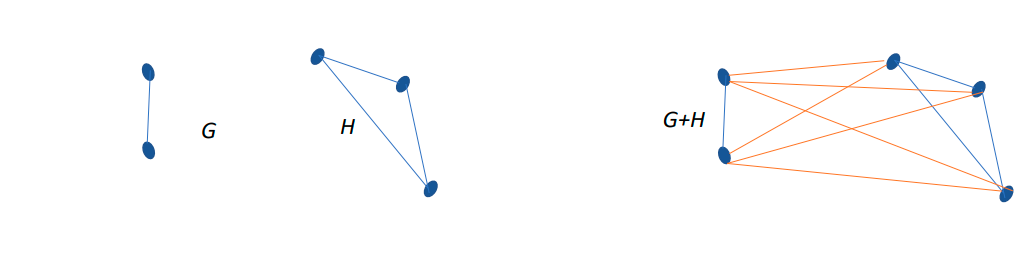
\includegraphics[width=\textwidth]{suma-grafos.PNG}

\subsubsection*{Definición 22. Complemento}
El complemento de G (grafo simple sin lazos no dirigido), que se denota $G^C$ o $\bar{G}$
es el subgrafo de $K_n$ formado por los n vértices de G y todas las aristas que no estan en G.

\subsubsection*{\hl{Definicion 23. Isomorfismo de Grafos}}
Sean $G_1(V_1, E_1)$ y $G_2(V_2, E_2)$ dos grafos no dirigidos, una función $f: V_1 \rightarrow V_2$ es un isomorfismo de grafos si:
\begin{enumerate}
    \item $f$ es biyectiva
    \item $\forall a,b \in V_1 \comma {a,b} \in E_1 \Leftrightarrows {f(a), f(b)} \in E_2$ (Preserva adyacencias, es decir tienen la misma matriz de adyacencia)
\end{enumerate}
Cuando existe dicha funcion, $G_1$ y $G_2$ son grafos isomorfos.
Cada clase de equivalencia se llama tipo de isomorfismo.
\\\underline{Notación:} $G_1 \eqsim G_2$.
\\\underline{Apuntes}: Básicamente, "dos grafos son isomorfos si son el mismo grafo dibujado distinto".

\subsubsection*{Definición 24. Camino}
Un camino desde el vértice $v_0$ al vértice $v_n$ es una secuencia alternada $w =< v_0,e_1,v_1,e_2,...,v_{n-1},e_n,v_n>$ de vértices y aristas donde $e_i=\{v_{i-1}, v_i\}$ con $i = 1,...,n$.
\\\underline{Notación}: camino $v_0 - v_n$
\\\underline{Apuntes}:
\begin{itemize}
    \item Puedo repetir vértices o aristas pero NO puedo saltearme vértices.
    \item Los caminos pueden indicarse nombrando sólo la secuencia de vértices si el grafo es simple de lo contrario hay que indicar las aristas.
    También podemos indicarlos mostrando la secuencia de aristas que recorre el camino. 
    Si lo único que interesa es decir que hay un camino entre un par de vértices podemos decir camino $v_0 - v_n$.
\end{itemize}

\subsubsection*{Definición 25. Camino directo}
Un camino directo en un digrafo de $v_0$ a $v_n$ es una secuencia alternada $w =< v_0,e_1,v_1,e_2,...,v_{n-1},e_n,v_n>$ de vértices y aristas donde $e_i=(v_{i-1}, v_i)$ con $i = 1,...,n$.
\\\underline{Notación}: camino directo $v_0 - v_n$
\\\underline{Apuntes}:
\begin{itemize}
    \item No es un camino directo si las flechas no me llevan. Por lo tanto puedo repetir vértices siempre y cuando la dirección de las aristas me lo permitan.
\end{itemize}

\subsubsection*{Definción 26. Longitud}
La longitud de un camino o camino directo es el numero de aristas que recorre el camino.

\subsubsection*{Definción 27. Cerrado}
Un camino o camino directo $x-y$ es cerrado si $x=y$, de lo contrario es abierto.

\subsubsection*{Definción 28. Concatencación}
La concatenación de dos caminos $w_1 =< v_0,e_1,v_1,e_2,...,v_{k-1},e_k,v_k>$ y $w_2 =< v_k,e_{k+1},v_{k+1},e_{k+2},...,v_{n-1},e_n,v_n>$ tal que $w_2$ empieza donde termina $w_1$ es el camino $w_1$ o $w_2 = < v_0,e_1,v_1,e_2,...,v_{n-1},e_n,v_n>$.
\\\underline{Notación}: camino $v_0 - v_n$
\\\underline{Apuntes}:
\begin{itemize}
    \item Para poder concatenar grafos/subgrafos, TIENEN que tener vértices en común.
    \item La longitud final (i.e. luego de concatenar) es: $\#E(w_1) + \#E(w_2)$
\end{itemize}

\subsubsection*{Definción 29. Subcamino}
Un subcamino de $w =< v_0,e_1,v_1,e_2,...,v_{n-1},e_n,v_n>$ es una subsecuencia de entradas consecutivas $s =< v_j,e_{j+1},v_{j+1},e_{j+2},...,v_{k-1},e_k,v_k>$ con $0 \leq j \leq k \leq n$ que comienza y termina en un vértice.
Un subcamino es en sí mismo un camino.
\\\underline{Apuntes}:
\begin{itemize}
    \item Todo camino es subcamino de si mismo.
    \item La longitud de un subcamino es $\leq$ a la del camino original.
\end{itemize}

\subsubsection*{Definción 30. Vértice alcanzable}
Un vértice $v$ es alcanzable desde un vértice $u$ si $\exists$ un camino $u-v$.
\\\underline{Apuntes}:
\begin{itemize}
    \item Es una relación de equivalencia (en un grafo, no necesariamente en un digrafo). Por lo tanto es R, S y T.
    \item No quiere decir que hay una arista que une dos vértices, quiere decir que hay un camino entre ellos.
\end{itemize}

\subsubsection*{Definición 31. Conexidad}
Un grafo es conexo si $\forall$ par de vértices $u$ y $v$ hay un camino $u-v$. 
En otras palabras, "para todo par de vértices de un grafo siempre hay un camino que los une".
\begin{center}
    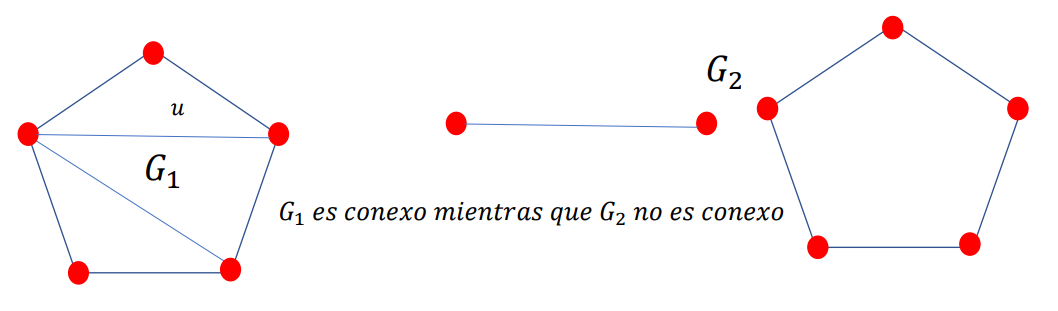
\includegraphics[width=.60\textwidth]{grafosConexos.PNG}
\end{center}

\subsubsection*{Definición 32. Digrafo Conexo}
Un digrafo es conexo si al considerarlo no dirigido es conexo (\emph{Conexidad debil}).
Un digrafo es \emph{fuertemente conexo} si todo par de vértices en el digrafo es mutuamente alcanzable.
Dos vértices $u$ y $v$ son mutuamente alcanzables si existen en el digrafo un camino directo $u - v$ y un camino directo $v - u$.
\\\underline{Apuntes}:
\begin{itemize}
    \item Si puedo probar que hay un \emph{camino directo cerrado} que pasa por todos los vértices del grafo, entonces el grafo es fuertemente conexo.
\end{itemize}

\subsubsection*{Definición 33. Distancia}
En un grafo la distancia de $s$ a $t$ es la longitud del camino mas corto de $s$ a $t$ o infinito si no hay camino.
\\En los digrafos la distancia directa es el largo del camino directo mas corto.
\\\underline{Notación}: $d(s,t)$

\subsubsection*{Definición 34. Reducción de un camino}
Dado un camino $w =<v_0,e_1,v_1,e_2,...,v_{n-1},e_n,v_n>$ que contiene un subcamino cerrado $\widetilde{w}=< v_k,e_{k+1},v_{k+1},e_{k+2},...,v_{m-1},e_m,v_m>$ la reducción de $w$ por $\widetilde{w}$ denotada por $w-\widetilde{w}$ es el camino $w-\widetilde{w}=<v_0,e_1,...,v_{k-1},e_k,v_k,v_{m+1},e_{m+1},...,v_{n-1},e_n,v_n>$, 
es decir que borra todas las aristas y vértices de $\widetilde{w}$ menos $v_k$.
\\En otras palabras, "reducir un camino es quitarle un subcamino cerrado (o parte de él) sin romper el camino".

\subsubsection*{Definición 35. Recorrido (Trail)}
Es un camino que no repite aristas.

\subsubsection*{Definición 36. Camino Simple (Path)}
Es un camino que no repite vértices.
\\\underline{Observación}: Todo camino simple es un recorrido, pero no al revés.

\subsubsection*{Definición 37. Circuito}
Es un recorrido cerrado.

\subsubsection*{Definición 38. Ciclo (Cycle)}
Es un camino simple cerrado en el que se repite un unico vértice (el primero, que es tambien el último).
\\\underline{Observación}: Todo ciclo es circuito, pero no al revés.

\subsubsection*{Definición 39. Colección de ciclos de aristas disjuntas} FINAL (no tan importante)
\\Una colección de ciclos de aristas disjuntas $G_1, G_2, ..., G_m$ es llamada una descomposición de un circuito $T$ si los $G_i$ son subcaminos
de $T$ y $E_T = \cup_1^m E_{Gi}$ y $\cap^m_1 E_{Gi} = \varnothing$.
\\\underline{Observación}:
\begin{itemize}
    \item SI HAY VÉRTICES DE GRADO IMPAR ENTONCES NO ES UN CIRCUITO.
    \item Todo circuito se puede descomponer en ciclos de aristas disjuntas.
    \item La colección de ciclos de aristas disjuntas NO es única.
\end{itemize}
\underline{Apuntes}: 
\begin{itemize}
    \item Ciclos de aristas disjuntas = Los ciclos no comparten aristas.
    \item Si tengo una colección de aristas disjuntas entonces puedo pasar por todos los vértices sin pasar por todas las aristas. Tambien puedo recorrer todas las aristas sin repetirlas.
\end{itemize} 
\begin{center}
    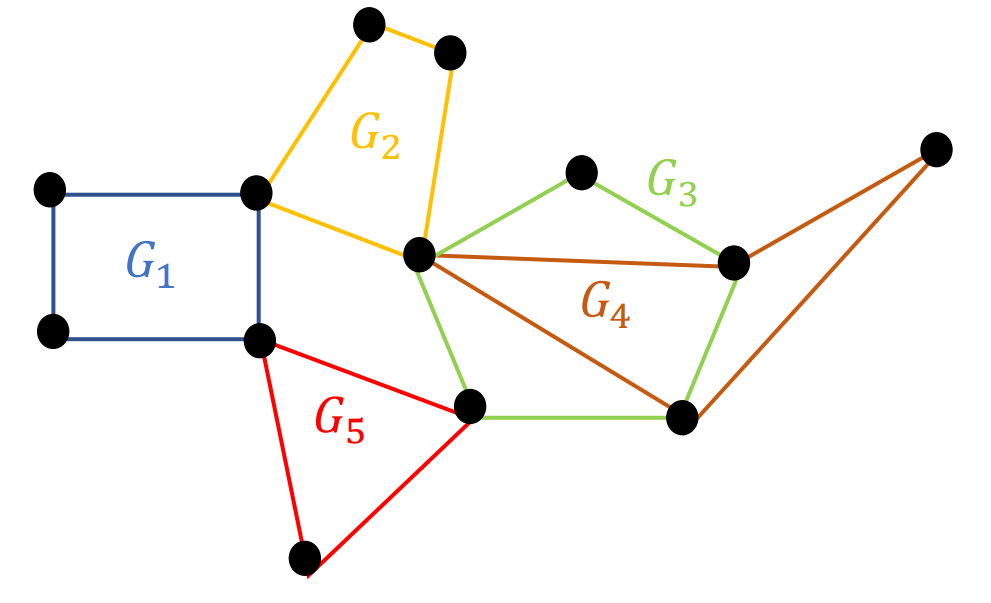
\includegraphics[width=.60\textwidth]{colCiclosAristasDisjuntas.PNG}
\end{center}
\nopagebreak[4]

\subsubsection*{Definición 40. Recorrido Euleriano}
Un recorrido euleriano en un grafo es un recorrido que contiene todas las aristas del grafo.
\begin{center}
    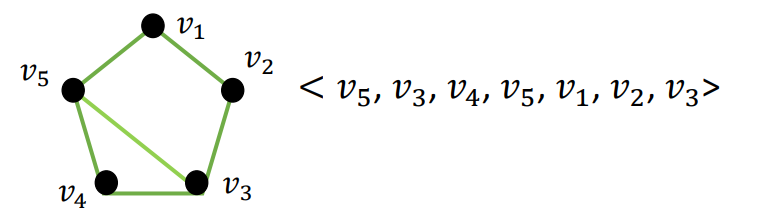
\includegraphics[width=.60\textwidth]{recorridoEuleriano.PNG}
\end{center}

\subsubsection*{Definición 41. Circuito Euleriano}
Un recorrido euleriano en un recorrido euleriano cerrado.

\subsubsection*{Definición 42. Grafo Euleriano}
Es un grafo que tiene un circuito euleriano.
\begin{center}
\begin{minipage}[c]{.45\textwidth}
    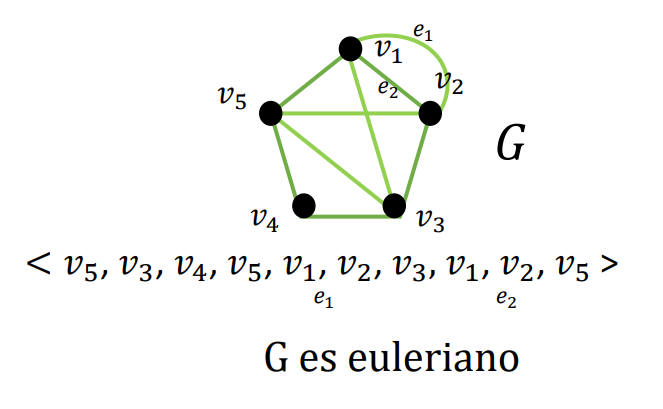
\includegraphics[width=\textwidth]{grafoEuleriano.PNG}
\end{minipage}
\end{center}

\subsubsection*{Definición 43. Camino Hamiltoniano}
Es un camino simple (no ciclo) en el grafo que contiene todos sus vértices.
\\\underline{Apuntes}:
\begin{itemize}
    \item Todos los $P_n$ son caminos hamiltonianos.
    \item Para buscar el ciclo de longitud mas corto, si encontras un subgrafo $K_3$ entonces ya está; sino buscas un $C_4$.
\end{itemize}
\begin{minipage}[C]{.30 \textwidth}
    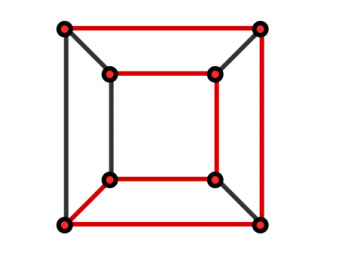
\includegraphics[width=\textwidth]{caminoHamiltoniano.PNG}
\end{minipage}
\begin{minipage}[C]{.70 \textwidth}
    \emph{El camino rojo marca el camino hamiltoniano}.
\end{minipage}

\subsubsection*{Definición 44. Ciclo Hamiltoniano}
\begin{minipage}[c]{.60\textwidth}
Si $G$ es un grafo o multigrafo y $\#V \geq 3$ decimos que $G$ tiene un ciclo hamiltoniano si existe un ciclo en $G$ que contenga cada vértice de $V$.
\\\underline{Apuntes}:
\begin{itemize}
    \item Cualquier $K_n$ tiene un ciclo hamiltoniano.
    \item La \emph{conexidad} es una condición necesaria pero no suficiente para que un grafo sea un ciclo hamiltoniano.
    \item \hl{Preg. de Final: Dibuje un grafo que sea un camino hamiltoniano pero no un ciclo hamiltoniano}. RESP: dibujar el moñito.
    \begin{center}
        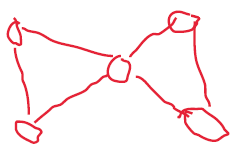
\includegraphics[width=.30\textwidth]{monioFinal.PNG}
    \end{center}
\end{itemize}
\end{minipage}
\begin{minipage}[c]{.40\textwidth}
    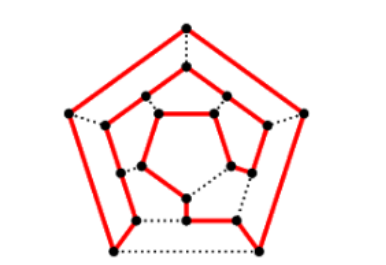
\includegraphics[width=\textwidth]{cicloHamiltoniano.PNG}
\end{minipage}

%---------------------------------------------------------------------------------------%
\subsection{Grafos Famosos}
\subsubsection*{$K_n$ (Completos)}
\begin{minipage}[c]{.45\textwidth}
\begin{itemize}
    \item $\#V = n$
    \item $\#E = \frac{n(n-1)}{2}$
    \item $n-1$ regular
    \item $K_n = K_{n-1} + v_n$
\end{itemize}
\end{minipage}
\begin{minipage}[c]{.45\textwidth}
    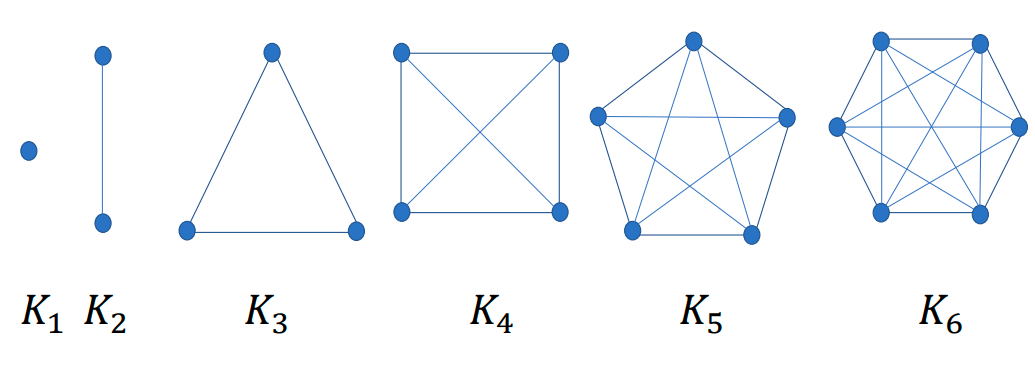
\includegraphics[width=\textwidth]{grafos completos.PNG}
\end{minipage}
\subsubsection*{$C_n$ (Ciclos)}
\begin{minipage}[c]{.45\textwidth}
\begin{itemize}
    \item $\#V = n$
    \item $\#E = n$
    \item 2-regular
    \item $C_n = P_n + e$ con $n \geq 3$
\end{itemize}
\end{minipage}
\begin{minipage}[c]{.45\textwidth}
    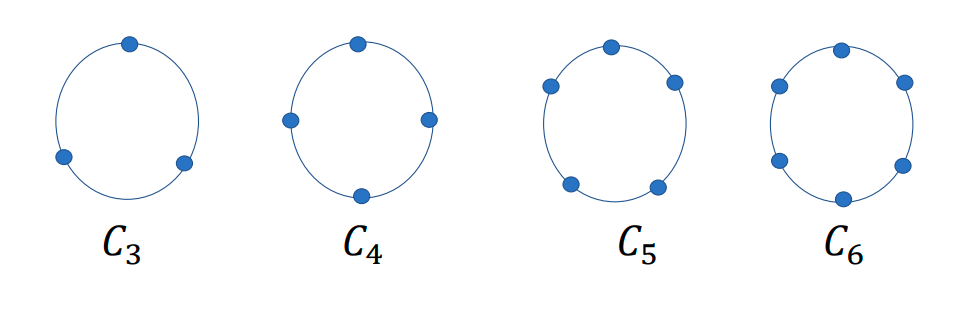
\includegraphics[width=\textwidth]{grafos ciclos.PNG}
\end{minipage}
\subsubsection*{$P_n$ (Caminos)}
\begin{minipage}[c]{.45\textwidth}
\begin{itemize}
    \item $\#V = n$
    \item $\#E = n - 1$
    \item No es regular salvo $P_1$ y $P_2$
\end{itemize}
\end{minipage}
\begin{minipage}[c]{.45\textwidth}
    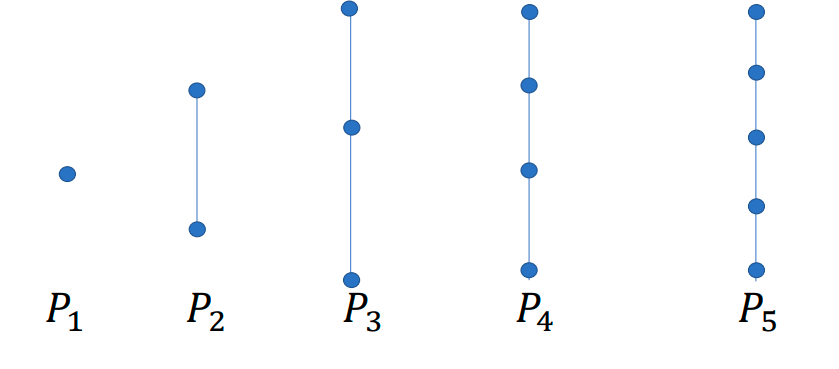
\includegraphics[width=\textwidth]{grafo camino.PNG}
\end{minipage}
\subsubsection*{$Q_n$ (Cubos)}
\begin{minipage}[c]{.45\textwidth}
\begin{itemize}
    \item $\#V = 2^n$
    \item $\#E = n2^{n-1}$
    \item n-regular
\end{itemize}
\end{minipage}
\begin{minipage}[c]{.45\textwidth}
    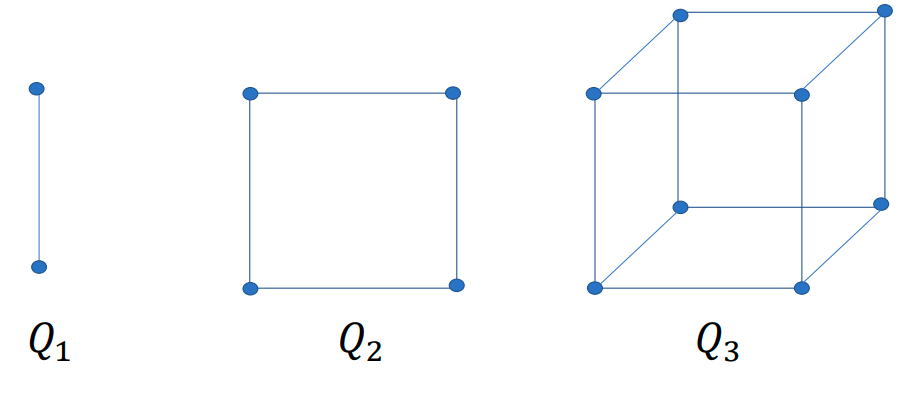
\includegraphics[width=\textwidth]{grafo cubo.PNG}
\end{minipage}

%---------------------------------------------------------------------------------------%
\subsection{Proposiciones}
\begin{enumerate}
    \item Sea el grafo $G(V,E)$ y sean $v_i \in V$ los vértices del grafo $G$, y $n = \#V$ entonces:
    \begin{equation*}
       \sumatoria{i=1}{n}g(v_i) \eq 2\#E \;\;\;\;\text{ (cada arista aporta 2 a la suma de grados)} 
    \end{equation*}
    \item La cantidad de vértices de grado impar es par.
    \item En un Digrafo la suma de los grados de entrada(o de salida) de los vértices es igual a la cantidad de aristas del digrafo.
    \item Todo camino abierto $x-y$ es un camino simple o contiene un subcamino cerrado.
    \item Sea $x-y$ un camino abierto, entonces $x-y$ es un camino simple o puede reducirse a un camino simple.
    \item \hl{Un grafo es bipartito $\Leftrightarrows$ el grafo no contiene ciclos de longitud impar}. 
    \item Todo circuito (consideramos al menos una arista) contiene un subcamino que es un ciclo.
    \item \hl{Todo circuito se puede descomponer en ciclos (aca consideramos a partir de $C_1$) de aristas disjuntas}.
    \item Sea $G$ un grafo o multigrafo no dirigido sin vértices aislados, entonces:
    \begin{center}
        \hl{$G$ es euleriano (en si mismo un circuito) $\Leftrightarrows$ $G$ es conexo y todos sus vertices tienen grado par}.
    \end{center}
    \item Sea $G$ un grafo o multigrafo no dirigido sin vértices aislados, entonces:
    \begin{center}
        \hl{$G$ tiene un recorrido euleriano (no circuito) $\Leftrightarrows$ $G$ es conexo y tiene exactamente 2 vertices de grado impar}.
    \end{center}
\end{enumerate}

%---------------------------------------------------------------------------------------%
%---------------------------------------------------------------------------------------%
\newpage
\section{Conexidad}
\bld{TODO SIN LAZOS}
\subsection{Definiciones Previas}
\subsubsection*{Definición 1. Componente de un grafo}
Se llama \emph{componente de un grafo} a un subgrafo conexo maximal del mismo o a los vértices aislados.
Es decir, si $H$ es una componente entonces no es un subgrafo propio de ninguna subgrafo conexo de $G$.
\begin{center}
    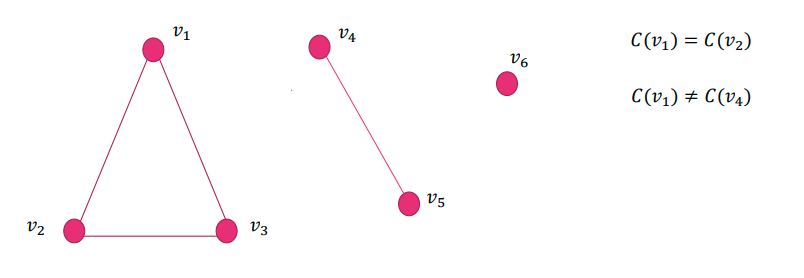
\includegraphics[width=.60\textwidth]{componenteGrafo.PNG}
\end{center}

\subsubsection*{Definición 2. Componente de un vértice}
Es el subgrafo inducido por todos los vértices alcanzables por $v$.
\\\underline{Notación}: $C(v)$
\\\underline{Observaciones}:
\begin{itemize}
    \item Si definimos $X \sim Y$ ($X$ se relaciona con $Y$), si $Y$ es alcanzable por $X$ (en un grafo) $\Rightarrows$ es una relación de equivalencia.
    \item Si $x \in C(v) \Rightarrows C(x) = C(v)$. Básicamente da lo mismo como llames a la componente.
\end{itemize}

\subsubsection*{\hl{Definicion 3. Vertice de corte/Punto de articulacion}}
Un vértice es de corte en un grafo $G$, si la cantidad de componentes conexas de $G -\{v\}$ es mayor que la cantidad de componentes conexas de $G$.
\\En otras palabras, es vértice de corte si cuando lo saco tengo mas componentes que antes. 
\begin{center}
    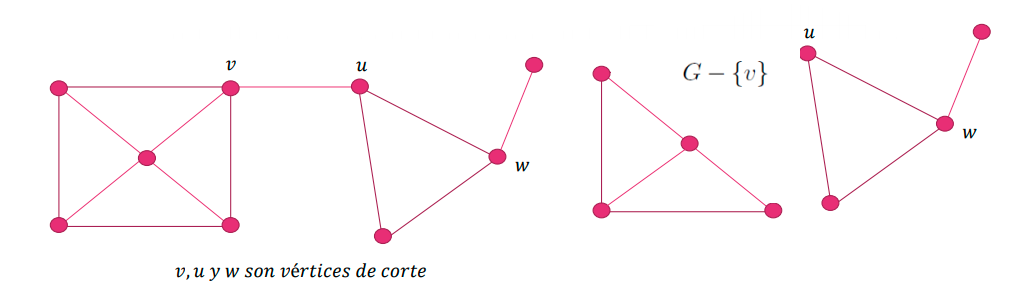
\includegraphics[width=.70\textwidth]{verticeCorte.PNG}
\end{center}
\leavevmode\\\fbox{\parbox{\dimexpr\linewidth-2\fboxsep-2\fboxrule\relax}
{\centering \underline{\hl{Teorema}}
   \\En un grafo conexo $G$, $v$ es vértice de corte $\Leftrightarrows \exists u\comma \in V_G\comma u\neq v \neq w \tq$ todo camino de $u-w$ contiene a $v$.
}}

\subsubsection*{Definición 4. Arista de corte/Arista puente}
Una arista $e$ es de corte, si la cantidad de componentes conexas de $G - \{e\}$ es mayor que la cantidad de componenetes conexas de $G$.
\begin{center}
    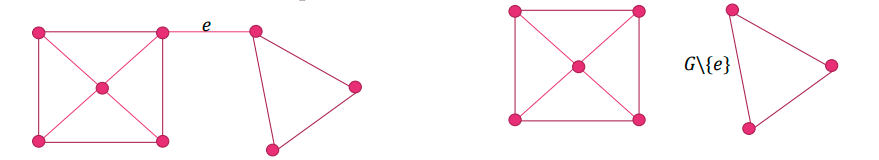
\includegraphics[width=.70\textwidth]{aristaCorte.PNG}
\end{center}
\underline{Observación}
\begin{itemize}
    \item Si tenemos la arista de corte $e = \{u,v\}$, entonces $v$ es vértice de corte si $g(v) \gneq 1$.
\end{itemize}
\leavevmode\\\fbox{\parbox{\dimexpr\linewidth-2\fboxsep-2\fboxrule\relax}
{\centering \underline{Teorema 2.A}
   \\En un grafo conexo $G$, $e$ es una arista de corte $\Leftrightarrows e \notin$ a un ciclo de $G$
}}

\subsubsection*{\hl{Definicion 5. Conexidad por vertices}}
Es la cantidad mínima de vértices que hay que remover del grafo $G$ para que deje de ser conexo o se transforme en el grafo trivial.
\\\underline{Notación}: $K_v(G)$
\\\underline{Observaciones}:
\begin{itemize}
    \item Si un grafo NO es conexo $\Rightarrows K_v(G) = 0$
    \item Si $K_v(G) \ge k \Rightarrows$ se dice que $G$ es $k$-conexo.
    \item Si un grafo es $k$-conexo $\Rightarrows \#V_G \gneq k$
\end{itemize}
\underline{Apuntes}:
\begin{itemize}
    \item $K_v(K_n) = n-1$
    \item Otra manera de ver la definición es, si un grafo es $k$-conexo, puedo sacarle $k-1$ vertices y sigue siendo conexo.
    \item Si $K_v(G)=2$ podemos decir que es 2-conexo o 1-conexo(conexo), pero NO podemos decir que es 3-conexo.
    \item El grafo puede convertirse en el grafo trivial.
\end{itemize}
\leavevmode\\\\\fbox{\parbox{\dimexpr\linewidth-2\fboxsep-2\fboxrule\relax}
{\centering \underline{Teorema 2.B}
    \\Sea $G$ un grafo $k$-conexo con $k \geq 3 \Rightarrows G-e \comma e \in E_G$ es $(k-1)$-conexo.
}}
\leavevmode\\\\\fbox{\parbox{\dimexpr\linewidth-2\fboxsep-2\fboxrule\relax}
{\centering \underline{\hl{Corolarios T2.B}}
    \begin{enumerate}
        \item Sea $G$ $k$-conexo, y $S$ un conjunto de $(k-1)$ aristas $\Rightarrows G-S$ es conexo.
        \item Sea $G$ $k$-conexo, y $S$ un conjunto de $m \lneq k$  aristas $\Rightarrows G-S$ es $(k-m)$ conexo.
        \item Sea $G$ un grafo conexo, la conectividad por aristas es $\geq$ que la conectividad por vértices.
    \end{enumerate}
}}

\subsubsection*{Definición 6. vértice Interno}
Dado un camino simple $P$ en un grafo $G$, $v$ es vértice interno si no es ni el inicial ni el final.

\subsubsection*{Definición 7. Colección de caminos internamente disjuntos}
Sean $u, v$ vértices de $G$, una colección de caminos internamente disjuntos $u - v$ (simples) es un conjunto de caminos tales que ningún par de ellos tiene vértices internos en común.
\begin{center}
    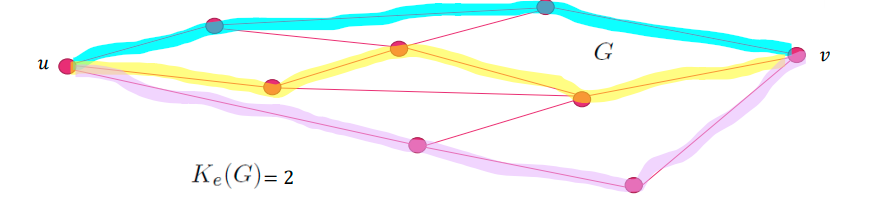
\includegraphics[width=.70\textwidth]{colCaminosInternamenteDisj.PNG}
\end{center}
\underline{Apuntes}:
\begin{itemize}
    \item Internamente Disjuntos = disjuntos por aristas Y por vértices.
    \item La máxima cantidad de caminos internamente disjuntos es el
     \\$min(K_v) = { u, v }$, siendo $u$ y $v$ los extremos del grafo.
    \begin{center}
        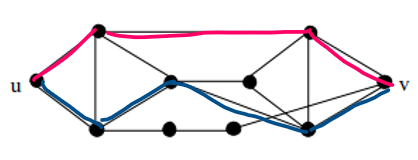
\includegraphics[width=.40\textwidth]{maxCantCaminosInternamenteDisjuntos.PNG}
    \end{center}
\end{itemize}
\underline{Posibles preguntas de Final}
\begin{itemize}
    \item $K_e(G)$ es igual al mínimo grado de G? NO
    \item Si G es $K_n$-regular entonces el $K_e(G)$ = grado? NO
    \item Dibujar un grafo $K_n$-regular con $K_e(G) = 2$
\end{itemize}

\subsubsection*{Definición 8. Conexidad por aristas}
Es la cantidad mínima de aristas que hay que remover del grafo $G$, para desconectarlo. 
\\\underline{Notación}: $K_e(G)$
\\\underline{Observaciones}:
\begin{itemize}
    \item $K_e(G) \ge k \Rightarrows$ se dice que $G$ es $k$-aristas conexo.
\end{itemize}
\underline{Apuntes}:
\begin{itemize}
    \item No se puede transformar en el grafo trivial (a diferencia de la conexidad por vértices)
\end{itemize}

\subsubsection*{Definición 9. Partición por corte de aristas}
$<X_1, X_2> : x_i$ es un conjunto de vértices del grafo $G$, que cumple: 
\begin{center}
    $X_1 \cup X_2 = V_G$ y $X_1 \cap X_2 = \varnothing$.
\end{center}
\leavevmode\\$<X_1, X_2> = \{e = \{u,v\} \tq u \in X_1 \wedge v \in X_2$
\begin{center}
    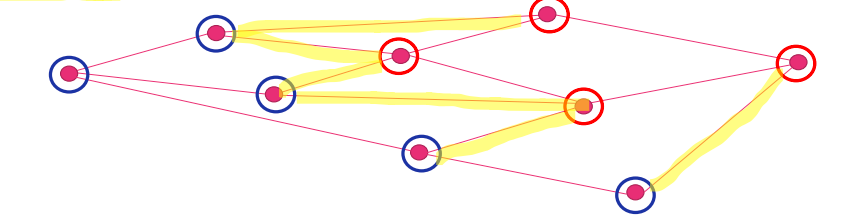
\includegraphics[width=.70\textwidth]{particionCorteAristas.PNG}
    donde $X_1$ son los vértices azules, $X_2$ los rojos y $<X_1,X_2>$ esta resaltado en amarillo.
\end{center}

\subsubsection*{Definición 10. Adición de un camino simple}
Dado un grafo $G$, adicionar un camino simple a $G$, es agregar un camino simple a $G$ entre un par de vértices de $G$, de modo que los vértices internos del camino no pertenezcan a $G$. 
\subsubsection*{Definición 11. Grafo Rueda}
Se obtiene un grafo rueda al sumarle un vértice a $C_{n-1}$
\begin{equation*}
    W_n = C_{n-1} + v \text{ con } n \geq 4 
\end{equation*}
\underline{Notación}: $W_n$
\begin{center}
    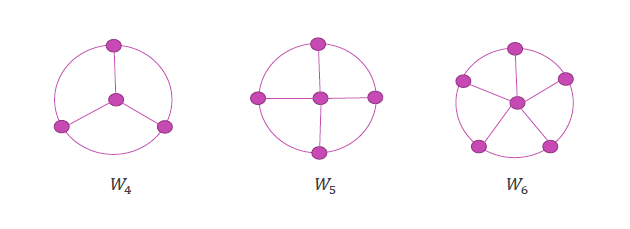
\includegraphics[width=.70\textwidth]{grafoRueda.PNG}
\end{center}

%---------------------------------------------------------------------------------------%
\subsection{Teoremas}
\subsubsection{Teorema de Whitney}
Sea $G$ un grafo conexo con 3 o mas vértices, entonces $G$ es 2-conexo $\Leftrightarrows \forall$par de vértices $u,v$ en $G$, hay por lo menos 2 caminos internamente disjuntos que los une.
\\\\\fbox{\parbox{\dimexpr\linewidth-2\fboxsep-2\fboxrule\relax}
{\centering \underline{\hl{Corolario del Teorema de Whitney}}
    \\Sea $G$ un grafo con, por lo menos 3 vértices $\Rightarrows$ $G$ es 2-conexo $\Leftrightarrows \forall$ par de vértices de $G$, hay un ciclo que los contiene.
}}
\leavevmode\\\\\fbox{\parbox{\dimexpr\linewidth-2\fboxsep-2\fboxrule\relax}
{\centering \underline{{Síntesis de Whitney}}
\\De un grafo $G$ desde un grafo $H$. Es una secuencia de grafos $G_0, ..., G_L$ donde $G_0 = H\comma G_L = G$ y $G_i$ se obtiene de adicionar un camino simple al $G_i - 1$.
\begin{center}
    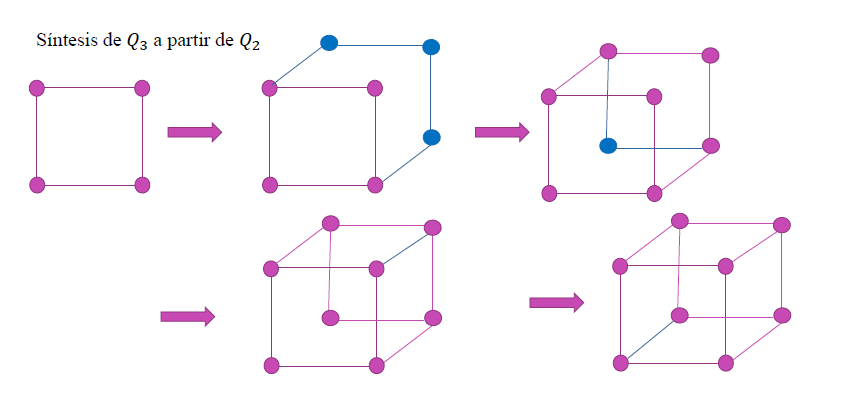
\includegraphics[width=.70\textwidth]{sintesisWhitney.PNG}
\end{center}
}}
\leavevmode\\\\\fbox{\parbox{\dimexpr\linewidth-2\fboxsep-2\fboxrule\relax}
{\centering \underline{Lemas}
\begin{enumerate}
    \item Sea $H$ un grafo 2-conexo $\Rightarrows$ el grafo $G$ que resulta de adicionar a $H$ un camino tambien es 2-conexo.
    \item Sea $H$ un subgrafo de un grafo $G$ 2-conexo, y sea $e$ una arista del $E_G - E_H \Rightarrows$ se puede adicionar un camino simple a $H$ que contiene dicha arista.
\end{enumerate}
}}
\leavevmode\\\\\fbox{\parbox{\dimexpr\linewidth-2\fboxsep-2\fboxrule\relax}
{\centering \underline{Teorema}
\\Un grafo $G$ es 2-conexo $\Leftrightarrows G$ es un ciclo o una síntesis de Whitney de un ciclo.
}}
\subsubsection*{\hl{Caracterizacion de los grafos 2-conexos}}
Sea $G$ un grafo conexo con por lo menos 3 vértices. Entonces las siguientes afirmaciones son equivalentes:
\begin{enumerate}
    \item El grafo $G$ es 2-conexo.
    \item $\forall$ par de vértices de $G$, $\exists$ un ciclo en $G$ que contiene a ambos.
    \item $\forall$ par de un vértice y una arista de $G$, $\exists$ un ciclo en $G$ que contiene a ambos.
    \item $\forall$ par de aristas de $G$, $\exists$ un ciclo en $G$ que contiene a ambas.
    \item $\forall$ par de vértices y una arista de $G$, $\exists$ un camino simple en $G$ que contiene a los 3.
    \item $\forall$ conjunto de 3 vértices distintos de $G$, $\exists$ un camino simple en $G$ que contiene a los 3.
    \item $\forall$ conjunto de 3 vértices distintos de $G$, $\exists$ un camino simple en $G$ que contiene a dos de ellos y no contiene al tercero.
\end{enumerate}

\subsubsection{Teorema de Tutte}
Es para reconocer grafos 3-conexos.
\\Un grafo $G$ es 3- conexo $\Leftrightarrows$ es un $W_n$ o se obtiene a partir de un $W_n$, por una secuencia de operaciones:
\begin{enumerate}
    \item Adición de una arista entre vértices de un grafo.
    \item Reemplazo de un vértice $v$ tal que $g(v) \geq 4$, por 2 vértices unidos por una arista, de modo que cada vértice adyacente al original, es ahora adyacente a
uno de los dos nuevos vértices, y sólo a uno, con la condición de que el grado
de cada nuevo vértice sea $g(vi) \geq 3$.
\end{enumerate}
\begin{center}
    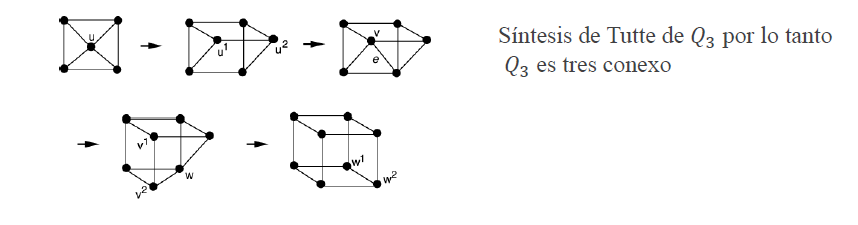
\includegraphics[width=\textwidth]{sintesisTutte.PNG}
\end{center}

\subsubsection{Teorema de Menger}
$G$ grafo conexo $u, v \in V_G$ no adyacentes $\Rightarrows$ la máxima cantidad de
caminos internamente disjuntos entre $u$ y $v$ es igual a la mínima cantidad de
vértices que hay que sacar para desconectar $u$ y $v$.

\subsubsection{Grafos de Harary}
\begin{equation*}
    H_{k,n} \text{ es el grafo de Harary $k$-conexo, con $n$ vertices y } \lceil\frac{kn}{2}\rceil \text{ aristas } (k \geq 2)
\end{equation*}
\subsubsection*{Caso 1. $k$ par}
Sea $k = 2r$
\\ Los vértices $i,j$ son adyacentes si $\underbrace{|j - i|_n}_{\text{min$\{|j - i|;\: n - |j - i|\}$}} \leq r$
\begin{center}
    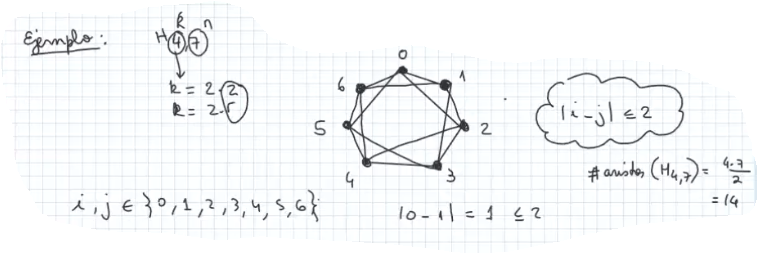
\includegraphics[width=\textwidth]{hararyC1.PNG}
\end{center}
\subsubsection*{Caso 2. $k$ impar y $n$ par}
Sea $k = 2r + 1$
\begin{enumerate}
    \item $H_{2r,n}$ (osea se cumple el Caso 1)
    \item Se agregan \emph{diámetros}, o sea: una arista entre los vértices $i$ e $i + \frac{n}{2}$ para $i = 0,1,...,\frac{n}{2} - 1$
\end{enumerate}
\begin{center}
    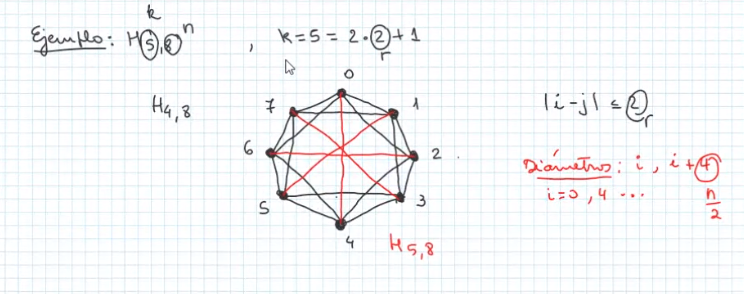
\includegraphics[width=\textwidth]{hararyC2.PNG}
\end{center}
\subsubsection*{Caso 3. $k$ impar y $n$ impar}
Sea $k = 2r + 1$
\begin{enumerate}
    \item $H_{2r,n}$ (osea se cumple el Caso 1)
    \item Se agregan \emph{cuasi-diámetros}, o sea:
    \begin{enumerate}
        \item Dibujar una arista desde 0 al $\frac{n-1}{2}$ y del 0 al $\frac{n+1}{2}$
        \item Dibujar una arista desde $i$ al $i + \frac{n+1}{2}$ para $i = 1, 2, ..., \frac{n-3}{2}$
    \end{enumerate}
\end{enumerate}
\begin{center}
    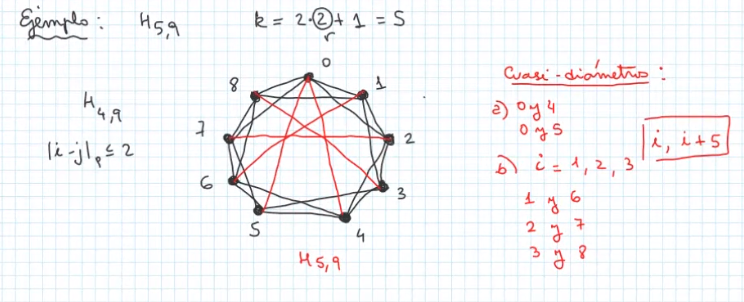
\includegraphics[width=\textwidth]{hararyC3.PNG}
\end{center}


%---------------------------------------------------------------------------------------%
\subsection{Proposiciones}
\begin{enumerate}
    \item Sea $G$ un grafo conexo y $\delta = min\{g(v_i)\} \;\forall v_i \in V_G \Rightarrows K_e(G) \leq \delta$.
    \item Se un grafo es $k$-aristas conexo $\Rightarrows$ toda partición por corte tiene, por lo menos, $k$ aristas.
    \item \hl{$\delta >= K_e(G) >= K_v(G) >= k$} \\(Posible pregunta de final: Dibujar un grafo donde se cumpla la desigualdad estricta)
    \begin{center}
        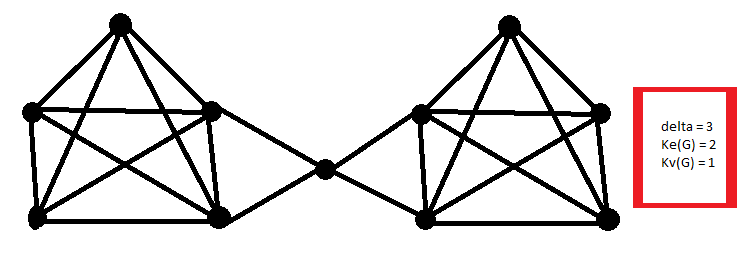
\includegraphics[width=.50\textwidth]{desigEstricta.PNG}
    \end{center}
    \item \hl{Sea $h_k(n)$ la minima cantidad de aristas necesarias para un grafo $k$-conexo con $n$-vertices $\Rightarrows h_k(n) \geq \lceil\frac{kn}{2}\rceil$}.
\end{enumerate}

%---------------------------------------------------------------------------------------%
%---------------------------------------------------------------------------------------%
\newpage
\section{Planaridad}
\subsection{Definiciones Previas}
\subsubsection*{Definición 1. Grafo Plano}
Un grafo es plano si puede dibujarse en el plano de modo que sus aristas se intersequen solo en los vértices de $G$. Es decir, es un grafo que no tiene aristas que se intersecan.
\\\emph{Función inmersión en el plano}:
\begin{equation*}
    i: G \rightarrow S
\end{equation*}
\begin{minipage}[C]{.50 \textwidth}
    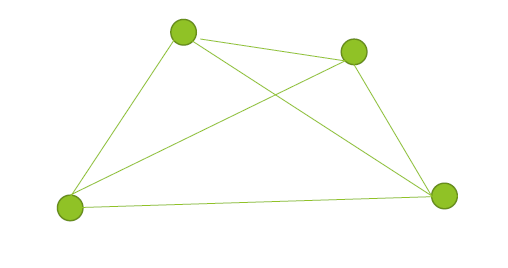
\includegraphics[width=.70\textwidth]{planaridad1.PNG}
\end{minipage}
\begin{minipage}[C]{.50 \textwidth}
    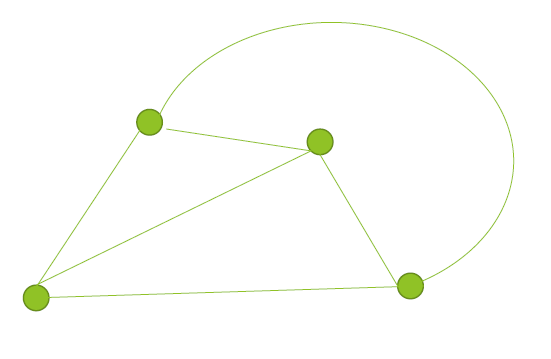
\includegraphics[width=.70\textwidth]{planaridad2.PNG}
\end{minipage}
\subsubsection*{Definición 2. Región}
Cuando realizamos la inmersión plana de un grafo $G$ el plano queda dividido en regiones contiguas llamadas caras o simplemente regiones.

\subsubsection*{Definición 3. Grado de una Región}
Número de aristas recorridas en un camino cerrado(el más corto) por las aristas de las fronteras de $R$.
\\Es decir, la cantidad de aristas que hay en la frontera de la región.
\\\underline{Notación}: $g(R)$

\subsubsection*{Definición 4. Aristas inseparables}
Sea $H$ un subgrafo de un grafo conexo $G$. Dos aristas $e_1$ y $e_2$ del conjunto de aristas $E_G - E_H$ son \emph{inseparables} por $H$ si existe un camino interno en $G$ que contiene
ambas aristas pero cuyos vértices internos no estan en $H$.
\\\underline{Observación}: La relación de inseparables por $H$ es una relación de equivalencia sobre $E_G - E_H$.
\begin{center}
    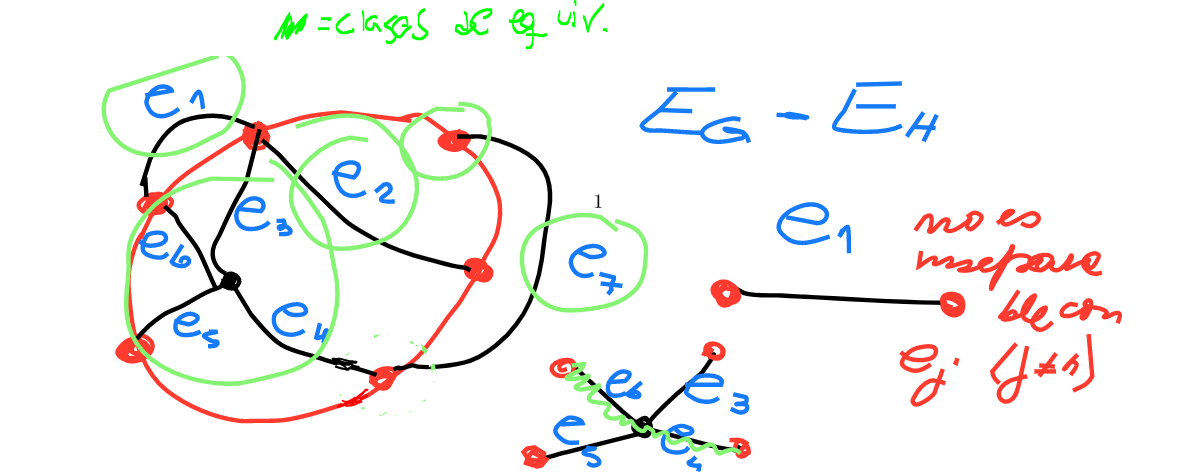
\includegraphics[width=.70\textwidth]{AristasInseparables.PNG}
\end{center}

\subsubsection*{Definición 5. Apéndice de un grafo}
Sea $H$ un subgrafo de un grafo $G$. Entonces un \emph{apéndice de $H$} es el subgrafo inducido sobre una clase de equivalencia de 
aristas de $E_G -E_H$ bajo la relación de inseparables.
\\Es decir, es el conjunto de aristas y vértices de una clase de equivalencia.
\\\underline{Observación}: Siempre se tiene que poder representar a todo el grafo G a partir de los apéndices mas H.
\begin{center}
    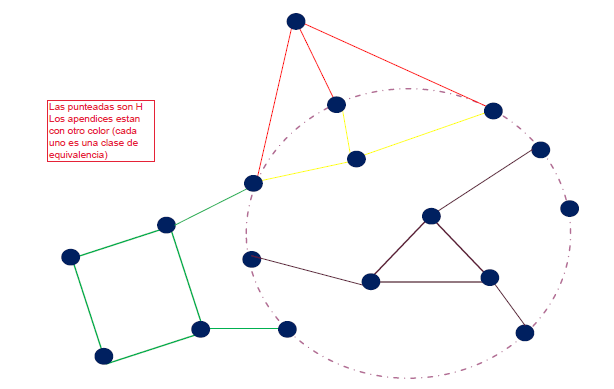
\includegraphics[width=.70\textwidth]{apendicesClasesEquiv.PNG}
\end{center}

\subsubsection*{Definición 6. Cuerda de un grafo}
Apéndice que tiene una sola arista. Une dos vértices de $H$ pero no esta en $H$.
\\Es decir, es una clase de equivalencia que tiene un sólo elemento (una sola arista).

\subsubsection*{Definición 7. Punto de contacto}
Sea $H$ un subgrafo de un grafo $G$ y sea $B$ un apéndice de $H$. Entonces un \emph{punto de contacto de $B$} es un vértice de $B \cap H$.
\begin{center}
    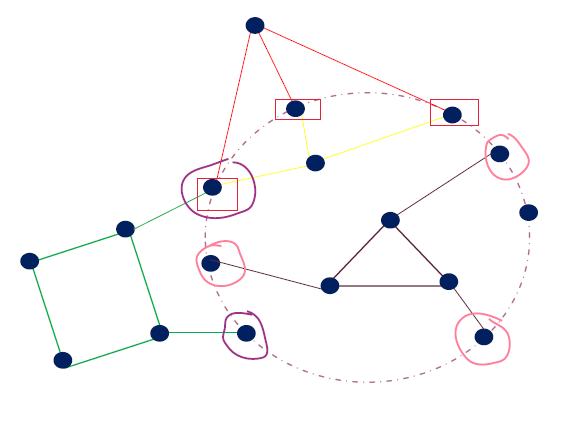
\includegraphics[width=.40\textwidth]{apendicesPtosContacto.PNG}
\end{center}

\subsubsection*{Definición 8. Superposición de apéndices}
Sea $C$ un ciclo en un grafo $G$. Los apéndices $B_1$ y $B_2$ de $C$ se superponen si ocurre alguna
de las siguientes condiciones:
\begin{enumerate}
    \item Dos puntos de contacto de $B_1$ alternan con 2 puntos de contacto de $B_2$ sobre un ciclo $C$.
    \item $B_1$ y $B_2$ tienen 3 puntos de contacto en común.
\end{enumerate}
\begin{center}
    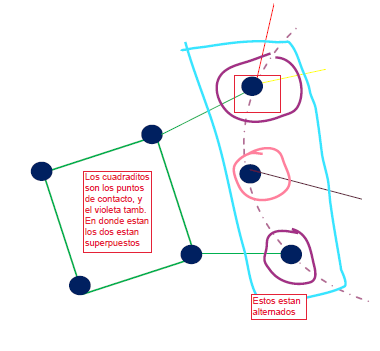
\includegraphics[width=.40\textwidth]{apendicesSuperpuestos.PNG}
\end{center}

%---------------------------------------------------------------------------------------%
\subsection{Algoritmo de Planaridad}
\begin{enumerate}
    \item Sea $H$ un subgrafo de un grafo $G$. En un dibujo plano de $H$, un \bld{apéndice de
$H$ no puede dibujarse en una región $R$} si la frontera de $R$ no contiene todos los
puntos de contacto del apéndice.
    \item  Sea $H$ un subgrafo de un grafo $G$. En un dibujo plano de $H$, un \bld{apéndice
de $H$ esta bloqueado} si dicho apéndice no puede dibujarse en ninguna region.
    \item Sea $H$ un subgrafo de un grafo $G$. En un dibujo de $H$ sobre alguna superficie,
un \bld{apéndice de $H$ esta forzado al interior de $R$}, si $R$ es la unica región cuya
frontera contiene todos los puntos de contacto del apéndice.
\end{enumerate}
\subsubsection*{Algoritmo}
Entrada: Un grafo $G$ 2-conexo.
\\Salida: Un dibujo plano de $G$ o Imprime que el grafo no es plano.
\\
\\1- Encuentre un ciclo arbitrario  $G_0$ en $G$ y dibújelo en el plano.
\\2- WHILE ($G_j \neq G$)
\\3- \{
\\4-   IF (algún apéndice está bloqueado) THEN PRINT "El grafo no es plano"; RETURN.
\\5-   IF (algún apéndice está forzado) THEN B:= dicho apéndice ELSE B:=cualquier apéndice.
\\6-   R:=región que contiene todos los puntos de contacto de B en su frontera.
\\7-   Seleccione un camino simple entre dos puntos de contacto de B y dibuje ese camino
    dentro de R para obtener $G_j + 1$.
\\8- \}
\\9- RETURN el dibujo plano de $G$

%---------------------------------------------------------------------------------------%
\subsection{Homeomorfismo}
Dos grafos $G$ y $H$ son homeomorfos si son isomorfos o si ambos pueden obtenerse del mismo grafo por una sucesión de subdivisiones elementales.
La relación de Homeomorfismo es una relación de equivalencia (es R, S y T).
\\\underline{Notación}: $G \sim_H H$
\\\underline{Observación}: El homeomorfismo NO MODIFICA la planaridad.

\subsubsection{Operaciones}
\subsubsection*{Subdivisión elemental de una arista}
Sea $e = \{u,v\}$ una arista del grafo $G$. Subdividir $e$ significa agregar $w$ a $V_G$ y reemplazar $e$ por $e_1 = \{u,w\}$ y $e_2 = \{u,w\}$

\subsubsection*{Remover débilmente un vértice}
Es la operación inversa a la anterior.
\\Sea $w$ un vértice de grado 2 en $G \tq e_1 = \{u,w\}$ y $e_2 = \{u,w\}$ son las aristas incidentes en él, 
remover débilmente $w$ significa sacar $w$ de $V_G$ y reemplazar $e_1$ y $e_2$ por la arista $e=\{u,v\}$.

%---------------------------------------------------------------------------------------%
\subsection{Teoremas}
\subsubsection{Teorema de Euler} \hl{FINAL}
Sea un grafo $G$ plano, conexo con $v$ vértices, $e$ aristas y $r$ el número de
regiones en el plano determinadas por una inmersión plana de $G$
\begin{equation*}
    \Rightarrows v - e + r = 2
\end{equation*}
\underline{Nota}: Cuenta como región infinita la región exterior al grafo.

\subsubsection{Teorema}
Si el grafo $G$ contiene un subgrafo $H$ que no es plano $\Rightarrows G$ no es plano.

\subsubsection{Teorema de Kuratowski}
Un grafo no es plano $\Leftrightarrows$ contiene un subgrafo homeomorfo $K_5$ o $K_{3,3}$.

%---------------------------------------------------------------------------------------%
\subsection{Proposiciones}
\begin{enumerate}
    \item Sea un grafo $G$ plano, conexo con $v$ vértices, $e$ aristas y $r$ el número de regiones en el plano determinadas por una inmersión plana de $G$
    \begin{equation*}
        \Rightarrows \sumatoria{i = 1}{r} g(R_i) = 2e
    \end{equation*}
    Cada arista pertenece a la frontera de dos regiones o se cuenta dos veces en la frontera de una misma región (vértice colgante)
    \item \hl{Sea $G$ un grafo plano, conexo, sin lazos, simple y con al menos 3 aristas}:
    \begin{equation*}
        \Rightarrows e \leq 3v - 6
    \end{equation*}
    \item \hl{Sea $G$ un grafo plano, conexo y bipartito}:
    \begin{equation*}
        \Rightarrows e \leq 2v - 4 \text{ con } e \geq 2
    \end{equation*}
    \underline{Nota}: 
    Si es bipartito conexo y plano $\Rightarrows$ es simple, conexo, plano y sin lazos (NO PASA VICEVERSA).
    \item Si el grafo $G$ es homeomorfo o isomorfo al grafo $H$, entonces:
    \begin{center}
        $H$ es plano $\Leftrightarrows G$ es plano
    \end{center}
    \item Sea $C$ un ciclo en un dibujo plano de un grafo y sean $B_1$ y $B_2$
apéndices superpuestos de $C$ $\Rightarrows$ Los apéndices NO pueden estar ambos del
mismo lado del ciclo en el plano.
    \item Sea $i : H \rightarrow S_0$ un dibujo plano de un subgrafo $H$ de un grafo $G$, tal que 
$H$ tiene un apéndice bloqueado $B \Rightarrows$ no es posible extender $i : H \rightarrow S_0$ a un 
dibujo plano de $G$.
    \item Un grafo es plano $\Leftrightarrows$ todos sus bloques son planos.
\end{enumerate}

%---------------------------------------------------------------------------------------%
\subsection{Posibles preguntas de Final}
\begin{enumerate}
    \item Dibujar un grafo donde se cumpla la condición del corolario de Euler y no sea plano.
    \\Respuesta:
    \begin{center}
        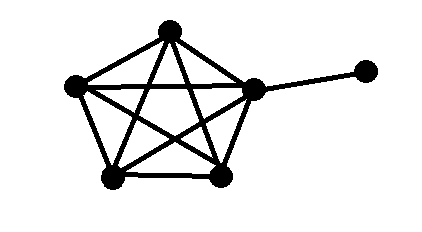
\includegraphics[width=.30\textwidth]{corolPeroNoPlano.PNG}
    \end{center}
    \item G plano conexo, simple, sin lazos entonces que se cumple? 
    \\Respuesta: Se cumple que la cantidad de aristas es menor/igual a 3v-6
\end{enumerate}

%---------------------------------------------------------------------------------------%
%---------------------------------------------------------------------------------------%
\newpage
\section{Bloques}
\subsection{Definiciones Previas}
\subsubsection*{Definición 1. Bloque}
Un bloque de un grafo sin lazos es un subgrafo conexo maximal $H$
tal que ningún vértice de H es un vértice de corte de $H$.
\\Si un bloque \emph{tiene por lo menos 3 vértices es 2-conexo}. Los únicos otros tipos
de bloque son aislados o dipolos.
\begin{center}
    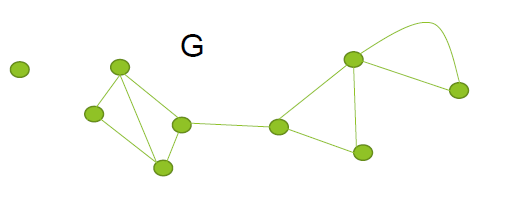
\includegraphics[width=.50\textwidth]{bloqueG.PNG}
    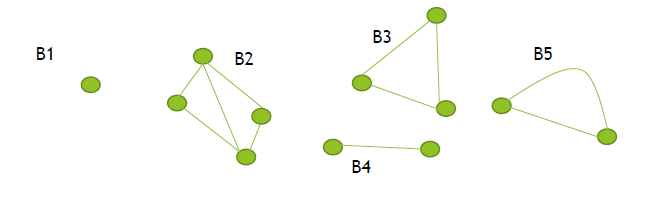
\includegraphics[width=.50\textwidth]{bloquesDeG.PNG}
\end{center}

\subsubsection*{Definición 2. Grafo Bloque}
Es un grafo  donde los vértices representan los bloques de $G$ y estos vértices estan unidos por una arista simple si los bloques en
$G$ tienen un vértice en común.
\\\underline{Notación}: BL(G)
\begin{center}
    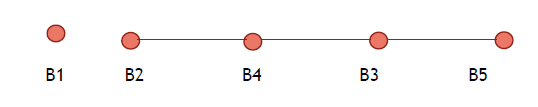
\includegraphics[width=.50\textwidth]{grafoBloqueG.PNG}
\end{center}

\subsubsection*{Definición 3. Bloque hoja}
Es un bloque que contiene exactamente un vértice de corte de $G$.
\\En la imagen anterior los Bloques Hoja son los vértices de grado 1, osea B2 y B5.

%---------------------------------------------------------------------------------------%
\subsection{Proposiciones}
\begin{enumerate}
    \item Todo grafo conexo $G$ no trivial contiene 2 o mas vértices que no son de corte.
    \item \hl{Dos bloques no conexos de un grafo $G$ deben tener como mucho un vertice en comun}.
    \item Si un grafo $G$ tiene por lo menos un vértice de corte $\Rightarrows G$ tiene por lo menos dos bloques hojas.
\end{enumerate}

%---------------------------------------------------------------------------------------%
\subsection{Corolarios}
\begin{enumerate}
    \item El conjunto de aristas de los bloques de un grafo $G$ es una partición del
conjunto $E_G$.
    \item Sea $x$ un vértice de $G \Rightarrows x$ es vértice de corte de $G \Leftrightarrows x$ esta en bloques diferentes de $G$.
    \item  Sean $B_1$ y $B_2$ bloques distintos de un grafo conexo $G$, $y_1$ e $y_2$ vértices de
$B_1$ y $B_2$ respectivamente tal que ninguno es vértice de corte de $G \Rightarrows y_1$ NO es
adyacente a $y_2$.
\end{enumerate}

%---------------------------------------------------------------------------------------%
%---------------------------------------------------------------------------------------%
\newpage
\section{Coloreo}
\bld{TODO SIN LAZOS}
\subsection{Definiciones Previas}
\subsubsection*{Definición 1. $k$-coloreo de vértices}
Es un coloreo que usa exactamente $k$ colores ($k \in \naturales$).

\subsubsection*{Definición 2. Coloreo propio}
Vértices adyacentes tienen colores distintos.

\subsubsection*{Definición 3. $k$-coloreable}
Un grafo $G$ es $k$-coloreable si tiene un $k$-coloreo propio
\begin{center}
    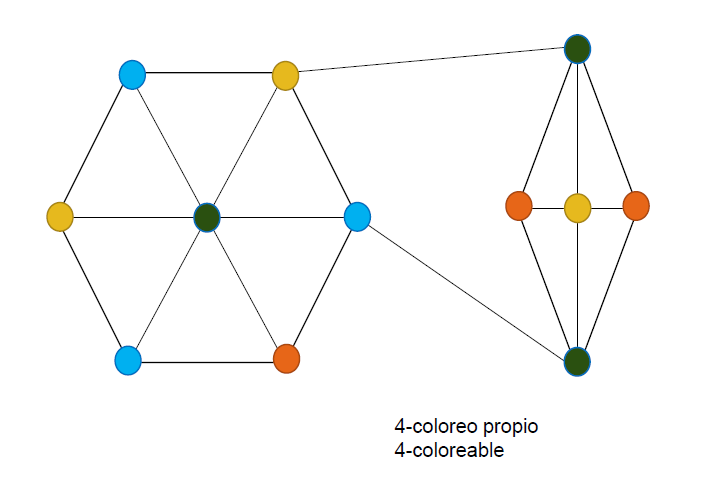
\includegraphics[width=.50\textwidth]{grafoNcoloreable.PNG}
\end{center}

\subsubsection*{Definición 4. Clase de color}
Es un subconjunto $V_G$ que tiene todos los vértices del mismo color.

\subsubsection*{Definición 5. Número Cromático}
Es el mínimo número de colores diferentes que se requiere para un coloreo propio.
\\\underline{Notacion}: $X(G) = k$ si G es $k$-cromatico

\subsubsection*{Definición 6. Clique}
Un clique en $G$ es un subconjunto maximal de vértices mutuamente adyacentes.
Es decir, es el $n$ de cada $K_n$ subgrafo de $G$.

\subsubsection*{Definición 7. Clique number}
Es el número de vértices del clique mas grande de $G$.
Es decir, es el subgrafo $K_n$ maximal con mayor $n$ que tiene $G$.
\\\underline{Notación}: $W(G)$

\subsubsection*{Definición 8. $k$-crítico}
Un grafo $G$ es $k$-crítico si $X(G) = k$ y $G-e$ es $(k-1)$-coloreable $\forall e \in E_G$

\subsubsection*{Definición 9. Obstrucción $k$-cromática}
Una obstrucción $k$-cromática es un subgrafo $H \tq  X(H) \gneq k$.
Entonces fuerza a todo grafo que lo contiene a tener $X(G) \gneq k$.

\subsubsection*{Definición 10. Conjunto de grafos críticos}
Un conjunto $\{G_j\}$ de grafos $(k + 1)$-críticos es un conjunto completo de
obstrucciones $k$-cromáticas con mínima cantidad de aristas, si todo grafo \\$(k + 1)$-cromático
contiene al menos un miembro de $\{G_j\}$ como subgrafo.
\begin{center}
    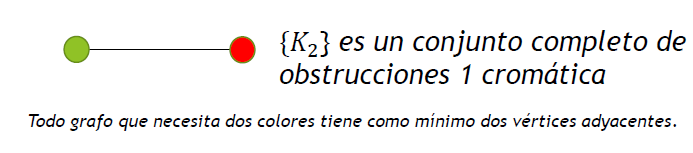
\includegraphics[width=.60\textwidth]{k2CjtoGrafoCritico.PNG}
\end{center} 

\subsubsection*{Definición 11. Conjunto de vértices independientes}
Un \emph{conjunto de vértices independientes de A} en un grafo, es un conjunto de vértices tales que
si $x$ e $y$ estan en $A$ en el grafo no hay arista con dichos vértices como extremos.

\subsubsection*{Definición 12. Independencia de $G$}
La \emph{independencia de $G$} es el máximo cardinal entre los conjuntos indepnendientes.
\\\underline{Notación}: $ind(G)$
%---------------------------------------------------------------------------------------%
\subsection{Proposiciones}
\begin{enumerate}
    \item Si $X(G)=k \Rightarrows G$ es $k$-coloreable pero no $(k-1)$-coloreable.
    \item Un grafo $G$ con $X(G) = 1$ no tiene aristas.
    \item Las aristas múltiples no afectan el coloreo pero los lazos lo impiden.
    \item Si $G$ es un grafo con $k$-vertices mutuamente adyacentes (i.e. $K_n$) $\Rightarrows X(G) \geq k$
    \item $K_n$ es $n$-cromático. Entonces, si $K_n$ es subgrafo de $G$ necesito como mínimo $n$ colores.
    \begin{center}
        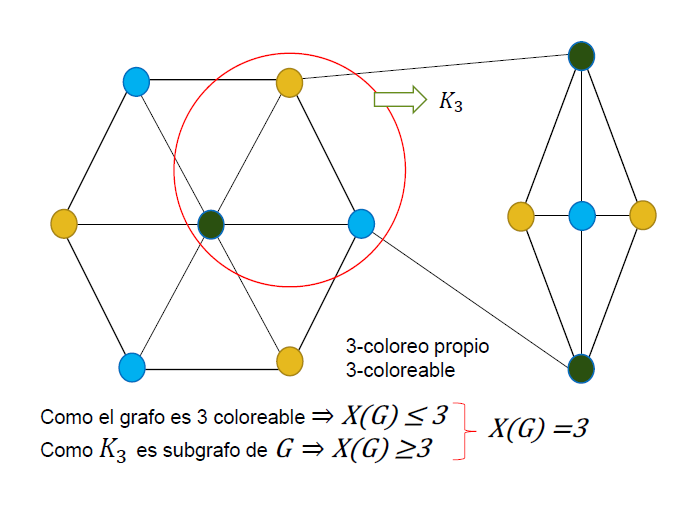
\includegraphics[width=.50\textwidth]{knNcoloreable.PNG}
    \end{center}
    \item Si $H$ es un subgrafo de $G \Rightarrows X(G) \geq X(H)$
    \item $X(G) \geq W(G)$
    \item $G$ y $H$ grafos $\Rightarrows X(G + H) = X(G) + X(H)$
    \item $G$ bipartito $\Rightarrows X(G) = 2$
    \item $G$ conexo, $k$-crítico y $v$ un vértice de $V_G \Rightarrows G-v$ es $(k-1)$-coloreable.
    \item \hl{$G$ conexo, $k$-critico $\Rightarrows g(v_i) \geq k - 1\; \forall v_i \in V_G$}
    \item Sea $G$ un grafo $(k+1)$-crítico $\Rightarrows G-e$ no es una obstrucción $k$-cromática $\Rightarrows G$ es una obstrucción $k$-cromática con mínima cantidad de aristas.
    \item Sea $G$ un grafo, entonces $X(G) \geq \lceil \frac{\#V_G}{ind(G)} \rceil$
    \item $X(G) \leq \delta_M(G) + 1$
    \item \bld{Teorema de Brooks}: $G$ no completo, $k$-regular, 2-conexo, con $k \geq 3$. Entonces
    $G$ tiene un vértice con dos vecinos no adyacentes entre ellos tal que $G - \{x,y\}$ es un grafo conexo.
    \item Sea $G$ un grafo simple, conexo, no completo con $\delta_M(G) \geq 3 \\\Rightarrows X(G) \leq \delta_M(G)$
\end{enumerate}

%---------------------------------------------------------------------------------------%
%---------------------------------------------------------------------------------------%
\newpage
\section{Grafo Dual}
Para construir un dual de una \emph{inmersión plana} de un grafo o multigrado plano $G$, colocamos un vértice 
dentro de cada región incluyendo la región infinita. Para cada arista compartida por dos regiones dibujamos una arista que une
los vértices que estan dentro de cada región. Si la frontera de la región tiene una
arista (entonces tiene un vértice colgante) que se recorre dos veces dibujamos un lazo en el vértice de dicha región.
\\\underline{Notación}: $G_d$
\subsection{Observaciones}
\begin{enumerate}
    \item Cada arista de $G$ se corresponde con una arista en $G_d$ y viceversa.
    \item Un vértice de grado 2 en $G$ origina en $G_d$ un par de aristas que unen los mismos vértices.
    \item Dado un lazo en $G$, si el interior de la región determinada por el lazo no
    contiene otro vértice o arista de $G$, entonces el lazo origina un vértice colgante en $G_d$ y viceversa.
    \item $G_d$ es un dual de $G$ y no el dual. No se mantiene el isomorfismo.
    \\\begin{minipage}{.45 \textwidth}
        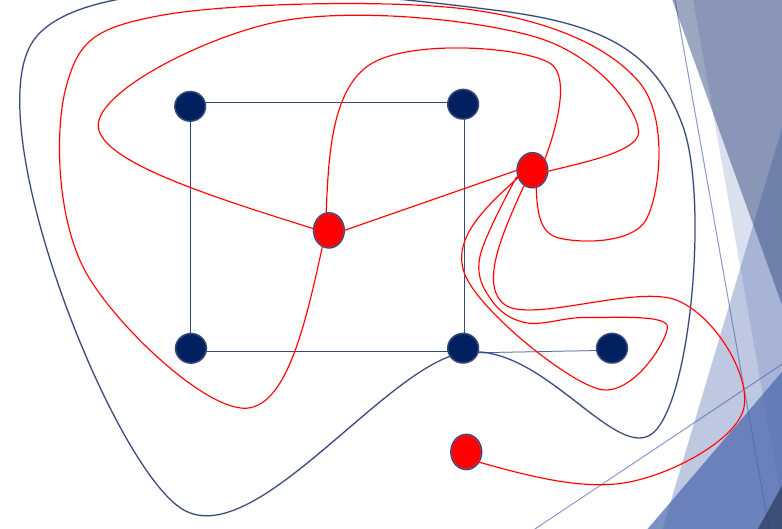
\includegraphics[width=\textwidth]{grafoDual1.PNG}
    \end{minipage}
    \begin{minipage}{.45 \textwidth}
        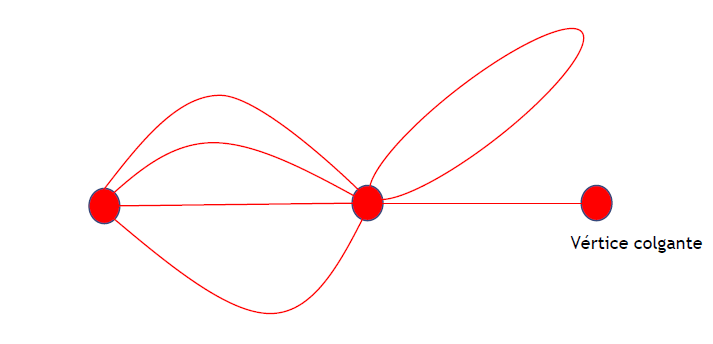
\includegraphics[width=\textwidth]{grafoDualB.PNG}
    \end{minipage}
    \\\begin{minipage}{.45 \textwidth}
        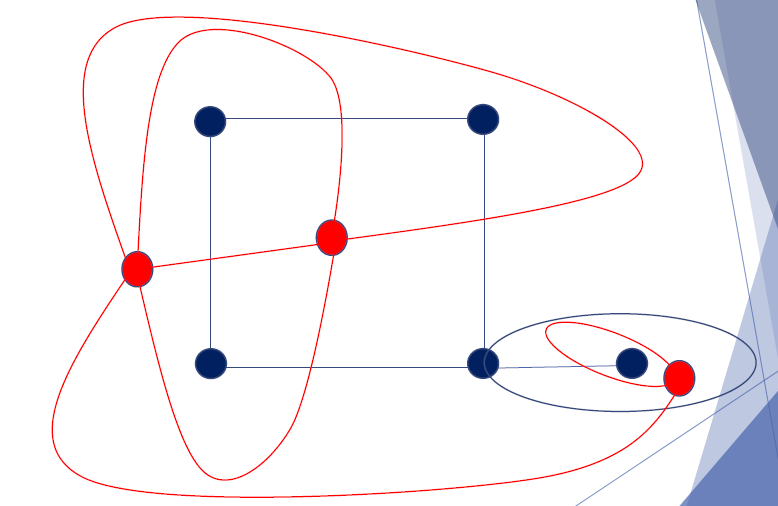
\includegraphics[width=\textwidth]{grafoDual.PNG}
    \end{minipage}
    \begin{minipage}{.45 \textwidth}
        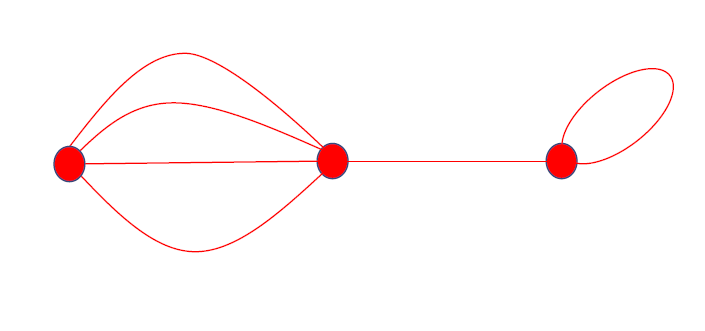
\includegraphics[width=\textwidth]{grafoDual2.PNG}
    \end{minipage}
    \item Los ciclos en $G$ de longitud $n$ se corresponden con un conjunto de corte de $n$ aristas en $G_d$ y viceversa.
    \item Un lazo en $G$ corresponde a un conjunto de corte (el conjunto de corte es de aristas)
    de una arista en $G_d$. Si el lazo no tiene nada dentro o todo el grafo estan dentro del lazo, queda un
    vértice colgante; si partes del grafo estan dentro del lazo y otras fuera queda un
    puente.
\end{enumerate}

%---------------------------------------------------------------------------------------%
%---------------------------------------------------------------------------------------%
\section{Complejidad}
\subsection{Definciones previas}
\subsubsection*{Definición 1. Algoritmo}
Es un conjunto de instrucciones perfectamente expresadas de tal modo que pueden ser
ejecutadas por una máquina o una persona, sin apelar a conocimientos adicionales a los
que requieran las mismas instrucciones ni al sentido común. La noción de algoritmo es la
de un procedimiento mecánico.
\\\underline{Propiedades}:
\begin{enumerate}
    \item \bld{Finitud}: Debe ser descripto por un texto finito.
    \item \bld{Efectividad}: Cada paso del algoritmo tiiene que podeer ser efectuado en la práctica.
    \item \bld{Terminación}: Tiene que parar en un número finito de pasos.
    \item \bld{Determinismo}: La secuencia de pasos tiene que estar unívocamente determinada para cada entrada.
\end{enumerate}

\subsubsection*{Definición 2. Complejidad}
La complejidad de un cálculo es la cantidad de recursos necesarios para efectuarlo.

\subsubsection*{Definición 3. Complejidad temporal}
La complejidad temporal de un cálculo es la cantidad de tiempo necesaria para efectuarlo.

\subsubsection*{Definición 4. Complejidad de los algoritmos}
La complejidad de un algoritmo es función de la longitud de la entrada, con lo cual se
puede analizar el peor caso, el mejor caso y el caso promedio. Para una definición formal
se adopta un punto de vista pesimista y se define la complejidad temporal del algoritmo
como su rendimiento en el peor caso. La complejidad de un problema es la complejidad
del algoritmo mas sencillo que lo resuelve.
\\\underline{Apuntes}:
\begin{enumerate}
    \item Si el $n$ de entrada es mayor $\Rightarrows$ la complejidad es mayor. FALSO
    \item Lo unico que contamos al evaluar la complejidad de un algoritmo son las \emph{comparaciones}.
\end{enumerate}
%---------------------------------------------------------------------------------------%
\subsection{Notación O mayúscula}
Es usada ampliamente para estimar el número de operaciones que un algoritmo usa
dependiendo del crecimiento de los datos de entrada.
\\\underline{Observaciones}:
\begin{outline}[enumerate]
    \1 Se tenemos dos funciones $f(n)$ y $g(n) \tq f(n) = O(h(n))$ y $g(n) = O(h(n)) \\\Rightarrows f(n)$ y $g(n)$ son del mismo orden.
    \1 Cuando $f(n)$ es $O(g(n))$ y $h(n)$ es una función que tiene valores absolutos mas grandes que $g(n)$ para valores mas grandes que $g(n)$
para valores mas grandes que $n \Rightarrows f(n) = O(h(n))$.
    \1 Cuando la función $O$ es usada, la funcion $g$ es escogida tan pequeña como sea posible.
    \1 $f_1(n)$ es $O(g_1(n))$ y $f_2(n)$ es $O(g_2(n))$. Entonces:
        \2 $(f_1 + f_2)(n)$ es de $O(max = \{ |g_1(n)|, |g_2(n)| \} )$
        \2 $(f_1 * f_2)(n)$ es de $O(g_1(n) * g_2(n))$
\end{outline}

%---------------------------------------------------------------------------------------%
%---------------------------------------------------------------------------------------%
\newpage
\section{Árboles}
\begin{center}
    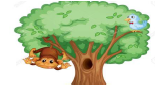
\includegraphics[width=.30\textwidth]{monitoXD.PNG}
\end{center}
TODO SIMPLE SIN LAZOS

\subsection{Definiciones Previas}
\subsubsection*{Definición 1. Árbol}
Un árbol es un grafo conexo que no tiene ciclos.
\begin{center}
    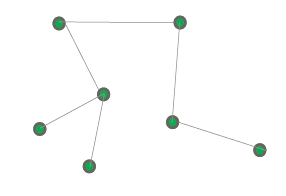
\includegraphics[width=.30\textwidth]{arbol.PNG}
\end{center}
\underline{Apuntes}:
\begin{enumerate}
    \item $K_1$ es el minimo arbol. $K_2$ es el minimo árbol con aristas.
\end{enumerate}

\subsubsection*{Definición 2. Arista ciclo}
Sea $e$ una arista de un grafo $G$ se llama arista ciclo si existe en $G$ un ciclo que la contiene.
\begin{center}
    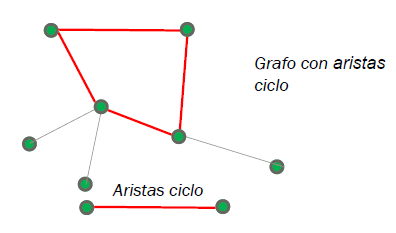
\includegraphics[width=.40\textwidth]{aristaCiclo.PNG}
\end{center}

\subsubsection*{Definición 3. Árbol dirigido}
Un árbol dirigido es un digafo cuyo grafo subyacente es un árbol.

\subsubsection*{Definición 4. Árbol con raiz}
Un árbol con raíz es un árbol dirigido con un vértice distinguido $r$ llamado tal que $\forall v \in V_G$ hay un camino directo de $r$ a $v$.
\begin{center}
    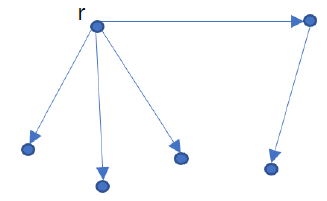
\includegraphics[width=.30\textwidth]{arbolConRaiz.PNG}
\end{center}

\subsubsection*{Definición 5. Profundidad}
Es un árbol con raíz la profundidad o nivel del vértice $v$ es su distancia a la raíz.
\begin{center}
    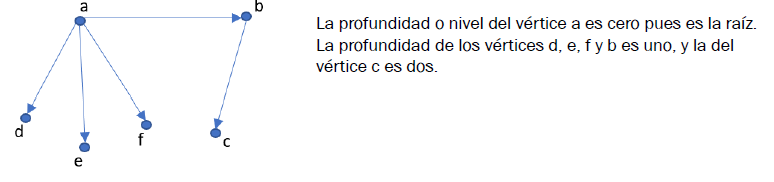
\includegraphics[width=.60\textwidth]{profundidadArbol.PNG}
\end{center}

\subsubsection*{Definición 6. Altura}
La altura de un árbol con raíz es la longitud del camino mas largo desde la raíz.
\begin{center}
    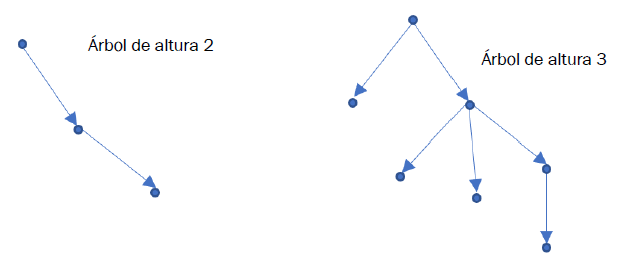
\includegraphics[width=.60\textwidth]{alturaArbol.PNG}
\end{center}

\subsubsection*{Definición 7. Padre - hijo}
Si el vértice $v$ es el que precede inmediatamente a $w$ en el camino directo $r - w$ entonces
$v$ es el padre de $w$ y $w$ es el hijo de $v$. Si dos vértices tienen el mismo padre, se llaman
hermanos.
\begin{center}
    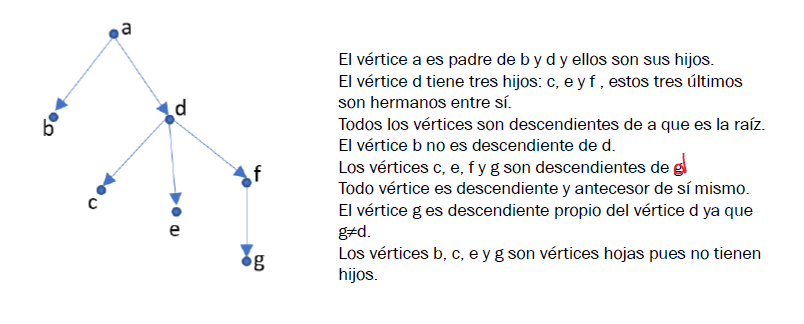
\includegraphics[width=.60\textwidth]{padreHijo.PNG}
\end{center}

\subsubsection*{Definición 8. Descendiente}
Un vértice $w$ es llamado descendiente de un vértice $v$, y $v$ es llamado \emph{antecesor de w}, si
$v$ esta en el unico camino $r - w$. Si $w \neq v$, $w$ es un descendiente propio de $v$, y $v$ un
antecesor propio de $w$.

\subsubsection*{Definición 9. Hoja}
Un vértice que no tiene hijos se llama hoja y un \emph{vértice interno} es un vértice que no es hoja.


\subsubsection*{Definición 10. Dibujo plano estándar}
Es dibujar la raíz arriba de todo y los vértices que estan a un mismo nivel horizontalmemte alineados.
\begin{center}
    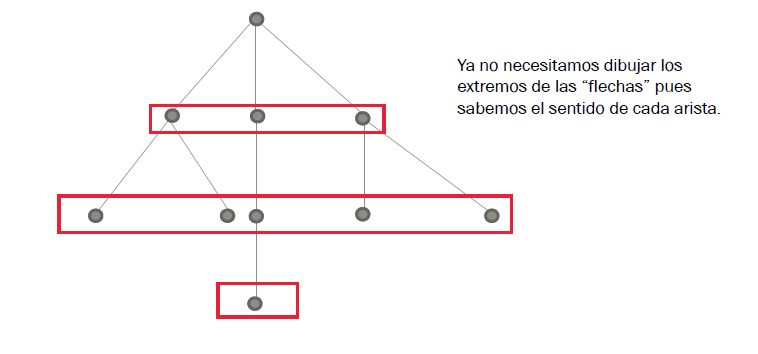
\includegraphics[width=.60\textwidth]{dibujoPlanoEstandar.PNG}
\end{center}

\subsubsection*{Definición 11. Árbol $m$-ario}
Un árbol $m$-ario con $m \geq 2$ es un árbol con raíz en el cual todo vertice tiene $m$ hijos o menos de $m$ hijos.
\begin{center}
    \includegraphics[width=.60\textwidth]{arbolMario.PNG}
\end{center}

\subsubsection*{Definición 12. Árbol $m$-ario completo}
Un árbol $m$-ario en el cual todos los vértices internos tienen exactamente $m$ hijos y todas las hojas tienen la misma profundidad.

\subsubsection*{Definición 13. Isomorfismo como árboles} 
Un árbol $m$-ario en el cual todos los vértices internos tienen exactamente $m$ hijos y todas las hojas tienen la misma profundidad.
\begin{center}
    \includegraphics[width=.60\textwidth]{isomorfismoArboles.PNG}
\end{center}

\subsubsection*{Definición 14. Árbol ordenado} 
Es un árbol con raíz en el cual cada hijo de cada vértice tiene asignado un orden fijo.

\subsubsection*{Definición 15. Árboles binarios} 
Un árbol binario es un árbol $2-ario$ en el cual cada hijo es deignado o hijo izquierdo o hijo derecho.
\begin{center}
    \includegraphics[width=.60\textwidth]{arbolBinario.PNG}
\end{center}

\subsubsection*{Definición 16. Subárbol}
El subárbol izquierdo (derecho) de un vértice $v$ en un árbol binario $T$ es el subárbol binario
recubridor del hijo izquierdo (derecho) y todos sus descendientes.
\begin{center}
    \includegraphics[width=.60\textwidth]{subarbol.PNG}
\end{center}

\subsubsection*{Definición 17. Código binario}
Un código binario es una asignación de símbolos a cadenas de bits. Cada cadena de bits se llama palabra del código.

\subsubsection*{Definición 18. Código prefijo}
Es un código binario con la siguiente propiedad: ninguna palabra del código es una subpalabra inicial de otra palabra del código.
\\\underline{\bld{Algoritmo de Huffman}}
\begin{center}
    \includegraphics[width=.60\textwidth]{algHuffman.PNG}
\end{center}

\subsubsection*{Definición 19. Pila}
Es una secuencia de elementos tal que cada nuevo elemento es agregado al final y se lo llama tope y un elemento es removido también del tope.
\\Last In First Out. LIFO.

\subsubsection*{Definición 20. Cola}
Es una secuencia de elementos tal que cada nuevo elemento es agregado al final y un elemento es removido del principio.
\\First In First Out. FIFO.

\subsubsection*{Definición 21. Árbol de Expresion}
Un árbol de expresión para una expresión aritmética es o un vértice etiquetado por un número o es un árbol que tiene un operador en la
raíz y los subárboles izquierdo y derecho son árboles de expresión.

\subsubsection*{Definición 22. Tabla de Acceso Aleatorio}
Es una tabla con dos columnas, en la primera se ponen los datos y en la segunda las claves.
La clave identifica la posición en la tabla del elemento que está en la misma fila.

\subsubsection*{Definición 23. Árbol Binario de Busqueda (BST)}
Es un árbol binario donde cada vértice tiene asignado una clave tal que la clave de un vértice v es más grande que
todas las de su subárbol izquierdo y más chica que todas las claves de su subárbol derecho.

\subsubsection*{Definición 24. Arista frontera}
Sea $T$ un árbol subgrafo de $G$, una arista $e=\{a,b\}$ se llama arista
frontera de $T$ si $a$ es un vértice de $T$ y $b$ es un vértice de $G$ que no está en $T$.

\subsubsection*{Definición 25. Árbol Binario Balanceado}
Si para todo vértice, el número de vértices de su subárbol izquierdo difiere a lo sumo en uno respecto al número de vértices
de su subárbol derecho.
\begin{center}
    \includegraphics[width=.50\textwidth]{arbolesBalanceados.PNG}
\end{center}
\underline{\bld{Operaciones}}
\begin{itemize}
    \item Realizar una busqueda
    \item Insertar
    \item Borrar
\end{itemize}

\subsubsection*{\hl{Definicion 26. $menor(w)$}}
\bld{PARCIAL}
\\$menor(w) = min\{dfnro(w), a\}$ siendo $a = min\{dfnro(v_j)\}$, si existe en $G-T$ una arista $\{v_j, desc(w)\}$
    \begin{center}
        \includegraphics[width=.80\textwidth]{menor(w).PNG}
    \end{center}

%---------------------------------------------------------------------------------------%
\subsection{Proposiciones}
\begin{enumerate}
    \item \hl{Sea $e$ una arista de un grafo conexo $G$ entonces $G - e$ es conexo $\Leftrightarrows e$ es una arista ciclo de $G$}.
    \\\\\fbox{\parbox{\dimexpr\linewidth-2\fboxsep-2\fboxrule\relax}
    {\centering \underline{Corolario P1.1}
    \\Una arista de un grafo es una arista de corte $\Leftrightarrows$ no es una arista ciclo.
    }}
    \\\\\fbox{\parbox{\dimexpr\linewidth-2\fboxsep-2\fboxrule\relax}
    {\centering \underline{Corolario P1.2}
    \\Sea $e$ cualquier arista de $G$. Entonces:
        \begin{equation*}
            k(G-e)
            \begin{cases}
                k(G) &\text{si } e \text{es una arista ciclo}\\
                k(G) + 1 &\text{en otro caso}
            \end{cases}
        \end{equation*}
    }}
    \item \hl{Todo arbol con por lo menos una arista tiene por lo menos dos vertices de grado 1}.
    \\\\\fbox{\parbox{\dimexpr\linewidth-2\fboxsep-2\fboxrule\relax}
    {\centering \underline{Corolario P2}
    \\Si el grado de todos los vértices de un grafo es $\geq 2 \Rightarrows$ el grafo debe contener al menos un ciclo.
    }}
    \item \hl{Todo arbol con $n$ vertices contiene exactamente $n-1$ aristas}.
    \\\\\fbox{\parbox{\dimexpr\linewidth-2\fboxsep-2\fboxrule\relax}
    {\centering \underline{Corolario P3.1}
    \\Un bosque $F$ con $n$ vértices tiene $n-k(G)$ aristas. Un \emph{bosque} es un conjunto de árboles.
    }}
    \\\\\fbox{\parbox{\dimexpr\linewidth-2\fboxsep-2\fboxrule\relax}
    {\centering \underline{Corolario P3.2}
    \\Un grafo bosque $G$ con $n$ vértices tiene por lo menos $n-k(G)$ aristas.
    }}
    \item \hl{Sea un grafo $G$ simple con $n$ vertices y $k$ componentes $\Rightarrows$ la cantidad de
aristas es $\# E_G \leq \frac{(n-k)(n-k+1)}{2}$}
    \\\\\fbox{\parbox{\dimexpr\linewidth-2\fboxsep-2\fboxrule\relax}
    {\centering \underline{\hl{Corolario P4}}
    \\Un grafo simple con $n$ vértices y más de $\frac{1}{2}(n-1)(n-2)$ aristas debe ser conexo.
    }}
    \item Un árbol $m$-ario tiene como mucho $m^k$ vértices en el nivel $k$.
    \item Sea $T$ un árbol en un grafo $G$ y sea $e$ una arista frontera de
$T \Rightarrows T + e$ es un árbol $T'$. 
    \item Sea $T$ un árbol recubridor producido por el algoritmo DFS en un grafo
no dirigido y sea $e=\{ x,y \}$ en $G-T \tq dfnro(x) \lneq dfnro(y) \Rightarrows x$ es un ancestro de $y$
en $T$.
    \item Cuando BFS es aplicado a un grafo no dirigido, los extremos de una
arista en $G-T$ están al mismo nivel o en niveles consecutivos.
    \item Sea $T$ un árbol que resulta de aplicar DFS a un grafo $G$ conexo,
    entonces un vértice $v$ de $T$ que no es raíz, es un vértice de corte de $G \Leftrightarrows v$
tiene un hijo $w$ tal que ningún descendiente de $w$ está unido a un ancestro
propio de $v$ por una arista en $G-T$.
    \begin{center}
        \includegraphics[width=.30\textwidth]{arbolesProp9.PNG}
    \end{center}
    \item \hl{Sea $T$ un arbol que resulta de aplicar DFS a un grafo $G$ conexo, entonces la raiz $r$ de $T$ es un vertice de corte de $G \Leftrightarrows r$ tiene mas de un hijo en $T$}.
    \item Sea $T$ un árbol que resulta de aplicar DFS a un grafo $G$ conexo,
    entonces un vértice $v$ de $T$ que no es raíz, es un vértice de corte de $G \Leftrightarrows v$
tiene un hijo $w$ tal que $menor(w) \geq dfnro(v)$.
    \item Sea $T_k$ el árbol de PRIM luego de $k$ iteraciones en el
algoritmo sobre el grafo $G$ conexo, donde $k \leq n -1$ ($n$ cant de vértices de $G$)
$\Rightarrows T_k$ es subárbol de un árbol mínimo recubridor $T$ de $G$.
\end{enumerate}

%---------------------------------------------------------------------------------------%
\subsection{Teoremas}
\subsubsection{Teorema 1}
\hl{Sea $T$ un grafo con $n$ vertices (sin lazos). Entonces las siguientes afirmaciones son equivalentes}:
\begin{enumerate}
    \item $T$ es un árbol
    \item $T$ no contiene ciclos y tiene $(n-1)$ aristas.
    \item $T$ es conexo y tiene $(n-1)$ aristas.
    \item $T$ es conexo y toda arista es una arista de corte.
    \item Todo par de vértices de $T$ estan conectados por exactamente un camino simple.
    \item $T$ no contiene ciclos y $T + e$ tiene exactamente un ciclo.
\end{enumerate}

\subsubsection{Teorema 2}
Sea $T$ un árbol con $n$ vértices y sea $G$ un gafo simple$\tq$
\begin{equation*}
    \delta_{min}(G) \geq n-1 \Rightarrows T \text{ es subgrafo de } G.
\end{equation*}

\subsubsection{Teorema 3}
Un árbol dirigido es repredentable como un árbol con raiz $\Leftrightarrows$ un vértice tiene grado de entrada 
0 y todos los demas grado de entrada 1.

\subsubsection{Teorema 4}
Sea $T$ un árbol $m$-ario con $n$ vértices y altura $h$. Entonces:
\begin{equation*}
    h+1 \leq n \leq \frac{m^{h+1}-1}{m-1}
\end{equation*}

\subsubsection{Teorema 5}
Un árbol binario completo de altura $h$ tiene $2^{h+1} - 1$ vértices.
\\\\\fbox{\parbox{\dimexpr\linewidth-2\fboxsep-2\fboxrule\relax}
{\centering \underline{Corolario T5}
\\Todo árbol binario de altura $h$ tiene a lo sumo $2^{h+1} -1$ vértices.
}}

%---------------------------------------------------------------------------------------%
\subsection{Algoritmos de Ordenación}
\subsubsection{Orden por Nivel}
El orden por nivel de un árbol ordenado es un listado de los vértices en orden creciente según la
profundidad, tal que los vértices que tienen la misma profundidad son listados acordes a su orden prescripto. De
arriba hacia abajo y de izquierda a derecha.
\\\underline{\bld{Algoritmo para Ordenar por Nivel}}
\begin{center}
    \includegraphics[width=.50\textwidth]{algOrdenPorNivel.PNG}
\end{center}

\subsubsection{Pre-Orden Izquierdo}
Hacemos una curva alrededor del árbol empezando por la raíz y dejando el árbol a la izquierda. 
A medida que vemos los vértices los vamos anotando en una lista.
\begin{center}
    \includegraphics[width=.60\textwidth]{algPreordenIzq.PNG}
\end{center}

\subsubsection{Post-Orden Izquierdo}
Hacemos una curva alrededor del árbol empezando por la raíz y dejando el árbol a la izquierda.
Anotamos los vértices la última vez que los vemos.
\begin{center}
    \includegraphics[width=.60\textwidth]{algPostOrdenIzq.PNG}
\end{center}
\underline{Apunte}: Es como hacer un Pre-Orden Derecho pero escrito de derecha a izquierda.

\subsubsection{In Orden}
Hacemos una curva alrededor del árbol empezando por la raíz y
dejando el árbol a la izquierda. Anotamos los vértices la segunda vez que los
vemos.
\begin{center}
    \includegraphics[width=.60\textwidth]{algInOrden.PNG}
\end{center}

\subsubsection{Depth First Search (DFS)}
\begin{center}
    \includegraphics[width=.60\textwidth]{algDFS.PNG}
\end{center}
\begin{minipage}{.5\textwidth}
    \begin{center}
        \includegraphics[width=.60\textwidth]{grafoDFS1.PNG}
    \end{center}
\end{minipage}
\begin{minipage}{.5\textwidth}
    \begin{center}
        \includegraphics[width=.40\textwidth]{grafoDFS2.PNG}
    \end{center}
\end{minipage}

\subsubsection{Breadth First Search (BFS)}
\begin{center}
    \includegraphics[width=.60\textwidth]{algBFS.PNG}
\end{center}
\begin{minipage}{.5\textwidth}
    \begin{center}
        \includegraphics[width=.60\textwidth]{grafoBFS1.PNG}
    \end{center}
\end{minipage}
\begin{minipage}{.5\textwidth}
    \begin{center}
        \includegraphics[width=.80\textwidth]{grafoBFS2.PNG}
    \end{center}
\end{minipage}
\subsubsection{Árbol Recubridor Mínimo}
Sea $G$ un grafo conexo ponderado encontrar un árbol recubridor de $G$ tal que el total de la suma de los pesos de las aristas sea mínimo.
    \begin{center}
        \includegraphics[width=.80\textwidth]{algPRIM.PNG}
    \end{center}
\underline{Ejemplo}:
    \begin{center}
        \includegraphics[width=.60\textwidth]{primEj.PNG}
    \end{center}

%---------------------------------------------------------------------------------------%
%---------------------------------------------------------------------------------------%
\newpage
\section{Redes de Flujo}
\subsection{Definiciones Previas}
\subsubsection*{Definición 1. Red}
Una red $N$ con una fuente simple (una sola) y un sumidero simple (uno solo) es un digrafo
conexo que tiene un vértice distinguido llamado fuente con grado de salida distinta de
cero y un vértice distinguido llamado sumidero con grado de entrada distinto de cero.
\\\underline{Notación}: red $f-s$
\\\underline{Apuntes}: \emph{Sólo la fuente genera productos y sólo el sumidero consume}.
\\\underline{Observación}: Si las capacidades son fraccionarias pueden ser transformadas en enteras
multiplicando por el MCM de los denominadores de las capacidades.

\subsubsection*{Definición 2. Red con Capacidad}
Una red con capacidad es un digrafo conexo tal que cada arco $e$ tiene
asignado una capacidad no negativa $cap(e)$ llamada \emph{capacidad del arco e}.
\\\underline{Notación}:
\begin{enumerate}
    \item $Sal(v) = \{ e \in E_N \tq$ la cola $(e) = v \}$
    \item $Ent(v) = \{ e \in E_N \tq$ la cabeza $(e) = v \}$
    \item $\langle X,Y \rangle = \{ e \in E_N \tq$ la cola $(e) \in X$ y la cabeza $e \in Y \}$
\end{enumerate}
\underline{Observación}: Si las capacidades son fraccionarias pueden ser transformadas en enteras
multiplicando por el MCM de los denominadores de las capacidades.
\begin{center}
    \includegraphics[width=.60\textwidth]{redDeFlujo.PNG}
\end{center}

\subsubsection*{Definición 3. Posible flujo}
Sea $N$ una red $f-s$ con capacidad, un \emph{posible flujo en $N$} es una función 
$f: E_N \rightarrow \reales^+$ que asigna un número real positivo $f(e)$ a cada arco $e$ tal que:
\begin{enumerate}
    \item \bld{Restricción de capacidad} \\$f(e) \leq cap(e)$ 
    \item \bld{Restricción de conservacion} \\$\sumatoria{e \in Ent(v)}{} f(e) = \sumatoria{e \in Sal(v)}{} f(e) \: \forall v \in V_N \tq v \neq f \lands v \neq s$ 
\end{enumerate}
\begin{center}
    \includegraphics[width=.70\textwidth]{posibleFlujo.PNG}
\end{center}

\subsubsection*{Definición 4. Valor de flujo}
El valor de flujo $f$ de una red con capacidad $N$ denotado $val(f)$ es el flujo neto que sale de la fuente.
\begin{equation*}
    val(f) = \sumatoria{e \in Ent(v)}{} f(e) - \sumatoria{e \in Sal(v)}{} f(e)
\end{equation*}

\subsubsection*{Definición 5. Flujo Máximo}
El flujo máximo $f^*$ en una red con capacidad es tal que $val(f) \leq val(f^*) \: \forall f \in N$

\subsubsection*{Definición 6. Corte en la red}
Sea $N$ una red $f-s$ y sea $V_f$ y $V_s$ una partición de los vértices de $N$ tal que $f \in V_f$ y
$s \in V_s$, entonces $\langle V_f, V_s \rangle$ se llama corte $f-s$ en la red.
\\\underline{Observación}: Note que el conjunto de aristas $Sal(f)$ es el corte $f-s$ $\langle f, V_N - \{f\} \rangle$ 
y que $Ent(s) = \langle V_N - \{s\}, s \rangle$.
\begin{center}
    \includegraphics[width=.60\textwidth]{corteEnLaRed.PNG}
\end{center}

\subsubsection*{Definición 7. Capacidad de un Corte}
La capacidad de un corte $\langle V_f,V_s \rangle$ denotada $cap\langle V_f, V_s \rangle$ es la suma de las capacidades de los
arcos en el corte $\langle V_f, V_s \rangle$. Es decir:
\begin{equation*}
    cap\langle V_f , V_s \rangle = \sumatoria{e \in \langle V_f, V_s \rangle}{} cap(e)
\end{equation*}

\subsubsection*{Definición 8. Corte Mínimo}
Un corte mínimo en la red $N$ es un corte con capacidad mínima.

\subsubsection*{Definición 9. Cuasi-camino}
Un \emph{cuasi-camino $f-s$} en una red $N$ es una secuencia alternada de vértices y aristas
$Q = \langle f = v_0, e_1, v_1, ..., v_k = s \rangle$ que forman un camino $f-s$ en el grafo subyacente
de $N$ (no importa el sentido de las flechas).
\\\underline{Notación}:
\begin{enumerate}
    \item \bld{Arco directo}: $v_{i - 1} \rightarrow v_i$
    \item \bld{Arco inverso}: $v_{i - 1} \leftarrow v_i$
\end{enumerate}

\subsubsection*{Definición 10. Camino de flujo aumentativo}
Sea $f$ un flujo en una red $N$. Un camino de flujo aumentativo $Q$ es un 
cuasi-camino $f-s$ en $N$ tal que el flujo de cada arco directo puede ser incrementado
y en cada arco inverso puede ser decrementado.
\begin{enumerate}
    \item $f(e) \lneq cap(e)$ si $e$ es un arco directo
    \item $f(e) \gneq 0$ si $e$ es un arco inverso
\end{enumerate}
\underline{Notación}:
\begin{enumerate}
    \item $\vartriangle e = cap(e) 0 f(e)$ si $e$ es un arco directo.
    \item $\vartriangle e = f(e)$ si $e$ es un arco inverso.
    \item $\vartriangle Q = min_{e \in Q}\{ \vartriangle e \}$
\end{enumerate}
\begin{center}
    \includegraphics[width=.60\textwidth]{caminoFlujoAumentativo.PNG}
\end{center}
\begin{center}
    \includegraphics[width=.60\textwidth]{caminoFlujoAumentativo2.PNG}
\end{center}
\begin{center}
    \includegraphics[width=.60\textwidth]{caminoFlujoAumentativo3.PNG}
\end{center}
\begin{center}
    \includegraphics[width=.60\textwidth]{caminoFlujoAumentativo4.PNG}
\end{center}

\subsection{Proposiciones}
\begin{enumerate}
    \item \hl{Sea $\langle V_f, V_s \rangle$ un corte de $f-s$ en la red $N$, entonces todo camino directo
    $f-s$ en $N$ contiene por lo menos un arco en este conjunto de corte}.
    \item \hl{Sea $f$ un flujo en una red $N$ y sea $\langle V_f, V_s \rangle$ un corte.  Entonces}:
    \begin{equation*}
        val(f) = \sumatoria{e \in \langle V_f, V_s \rangle}{} f(e) -\sumatoria{e \in \langle V_s, V_f \rangle}{} f(e) 
    \end{equation*}
\end{enumerate}
\leavevmode\\\fbox{\parbox{\dimexpr\linewidth-2\fboxsep-2\fboxrule\relax}
{\centering \underline{Corolario P2}
\\Sea $f$ un flujo en una red $f-s$. Entonces:
\begin{equation*}
    val(f) = \sumatoria{e \in Ent(s)}{} f(e) - \sumatoria{e \in Sal(s)}{} f(e)
\end{equation*}
\begin{center}
    \includegraphics[width=.60\textwidth]{corolarioValorDelFlujo.PNG}
\end{center}
}}

\subsection{Teoremas}
\subsubsection{Problema de Flujo y Corte Máximo}
\hl{Sea $f$ un flujo en una red $N$ y sea $\langle V_f, V_s \rangle$ un corte}. Entonces:
\begin{equation*}
    val(f) \leq cap \langle V_f, V_s \rangle
\end{equation*}
\leavevmode\\\fbox{\parbox{\dimexpr\linewidth-2\fboxsep-2\fboxrule\relax}
{\centering \underline{Corolario 1}
\\Sea $f^*$ un flujo máximo en una red $N$ y sea $K^*$ un corte mínimo en $N$.
Entonces el valor del flujo máximo es menor o igual que la capacidad mínima.
\begin{equation*}
    val(f) \leq cap(K^*)
\end{equation*}
}}
\leavevmode\\\\\fbox{\parbox{\dimexpr\linewidth-2\fboxsep-2\fboxrule\relax}
{\centering \underline{\hl{Corolario 2}}
\\Sea $f$ un flujo en ua red $N$ y sea $K$ un corte. Supongamos que $val(f) = cap(K)$. Entonces
$f$ es un flujo máximo y $K$ es un corte mínimo.
}}
\leavevmode\\\\\fbox{\parbox{\dimexpr\linewidth-2\fboxsep-2\fboxrule\relax}
{\centering \underline{Corolario 3}
\\Sea $\langle V_f , V_s \rangle$ un corte en la red $N$ y supongamos que $f$ es un flujo tal que:
\begin{enumerate}
    \item $f(e) = cap(e)$ si $e \in \langle V_f, V_s \rangle$
    \item $f(e) = 0$ si $e \in \langle V_s, V_f \rangle$
\end{enumerate}
Entonces $f$ es un flujo máximo y $\langle V_s, V_f \rangle$ es un corte mínimo.
}}

\subsubsection{Lema}
Sea $\langle V_f, V_s \rangle$ un corte $f - s$ en la red $N$. Entonces:
\begin{equation*}
    \cup_{v \in V_f} Sal(v) =  \langle V_f, V_f \rangle \cup \langle V_f, V_s \rangle
    \text{ y }
    \cup_{v \in V_f} Ent(v) =  \langle V_f, V_f \rangle \cup \langle V_s, V_f \rangle
\end{equation*}

\end{document}
